%% Copyright (C) 2009 by Tobias Elze
%% Journal of Vision LaTeX template version 1.0
%% This document may be used freely for your own submissions.

\documentclass{jov}
\usepackage{graphicx} % needed for figures
\usepackage{subcaption}
\usepackage{hyperref}
\usepackage{amsmath}
\usepackage{bbm}
\usepackage{amssymb}
\usepackage{comment}

\DeclareMathOperator*{\argmin}{arg\,min}

\begin{document}

\title{Luminance constancy under fixed geometry}
\abstract{The light that reflects off an object surface and is captured by our eyes varies significantly with its context. 
But, the human visual system has the ability to stably perceive the object's color invariant of the context variations. 
While this invariance detection ability is behaviorally very significant, its mechanism remains largely unknown. 
To understand the computational principles that lead to invariant color perception, 
here we study the perception of object light reflectance value (LRV) under variations in naturalistic scenes. 
Specifically, we study the effects of variations in reflectance and illumination spectra in a scene on the 
perceived LRV of a target object. 
We have developed a software that renders naturalistic multispectral images of 3D scenes.
The software provides precise control over the geometrical and spectral factors that make a scene. 
We label the rendered images with the luminance of a specific object in the scene. 
Next, we simulate the response of the retinal cones to these multispectral images using 
an accurate model of the early visual system. 
We then use supervised learning methods on these labeled cone responses to 
identify the computations that lead to accurate LRV estimation under changes in spectral condition. 
We show that if only either target or target and illumination spectra are allowed to vary, the standard luminance can be estimated through simple transformations of the cone responses. 
When all the spectra vary simultaneously, while it is not easy to recover the luminance through simple transformations, 
a decoding scheme that compares the light from the target and the surround, and properly adds the response of the L,M and  
S cones can recover the luminance within about 13\% RMSE.}

\author{Singh}{Vijay}
 {Computational Neuroscience Initiative}
 {and Department of Physics, University of Pennsylvania, PA, USA}
 {}{vsin@sas.upenn.edu}
 
 \author{Cottaris}{Nicolas P.}
 {}
 {Department of Psychology, University of Pennsylvania, PA, USA}
 {}{cottaris@sas.upenn.edu}
 
 \author{Heasly}{Benjamin S.}
 {}
 {Department of Psychology, University of Pennsylvania, PA, USA}
 {}{benjamin.heasly@gmail.com}
 
 \author{Brainard}{David H.}
 {}
 {Department of Psychology, University of Pennsylvania, PA, USA}
 {}{brainard@psych.upenn.edu}
 
 \author{Burge}{Johannes}
 {}
 {Department of Psychology, University of Pennsylvania, PA, USA}
 {}{jburge@psych.upenn.edu}

\keywords{color constancy, luminance constancy, supervised learning}

\maketitle

\section{Introduction}
The perceived color of an object has important behavioral implications, since color helps to identify objects and their properties \cite{Mollon89, Jacobs81}.
%The perceived color depends on the surface reflectance of the object, but it is not sensed directly. 
%Rather, it is computed by the brain starting with the retinal image of the light reflected from an object to the eye.
The computational challenge underlying object color perception is that the light reflected from an object depends not just on its surface reflectance, but also on object-extrinsic factors such as the illumination, the object's pose, and the position of the observer (Fig.~\ref{fig:introSchematic}).
To compute a perceptual representation of object color that is correlated with the object's physical surface reflectance, the brain must account for these object-extrinsic factors.
The ability of a visual system to compute a representation of object color that is stable against variation in object-extrinsic scene factors is called color constancy. 
Although human color constancy is by no means perfect, it is often very good \cite{FosterColorConstancy, BrainardColorConstancy}. 
In this paper, we consider the computational problem of color constancy, that is, how in principle could a visual system process the light reflected to the eye to produce percepts well-correlated with object surface reflectance.

Early work on computational color constancy considered a simplified case with multiple flat matte objects and a single spatially diffuse illuminant \cite{LandRetinex,Buchsbaum80,MaloneyWandell86}.
Subsequent computational work considered more complex geometries and incorporated probabilistic descriptions of the statistics of naturally occurring scenes \cite{funt1988color, D'ZmuraConstancy3, barron2012color, D'ZmuraIversonSinger,BrainardFreeman}.
A key insight from this computational work is that stable color descriptors of a target object cannot be obtained from the light reflected from the target object alone.
But, it is possible to obtain such descriptors by analyzing jointly the light reflected from all of the objects in the scene.
As a consequence, the performance of color constancy algorithms will be affected by variation in the surface reflectance of all of the objects in the scene \cite{BrainardWandellRetinex}, not just by variation in the illuminant; evaluation of constancy algorithms must include assessment of their performance with respect to both variation in the illumination and the surface reflectance of all of the scene objects \cite{BrainardWandellRetinex,BrainardFreeman}. 

% Figure 1: Introduction
\begin{figure}
\centering
\begin{subfigure}{0.4 \textwidth}
	\centering
	\caption{}
        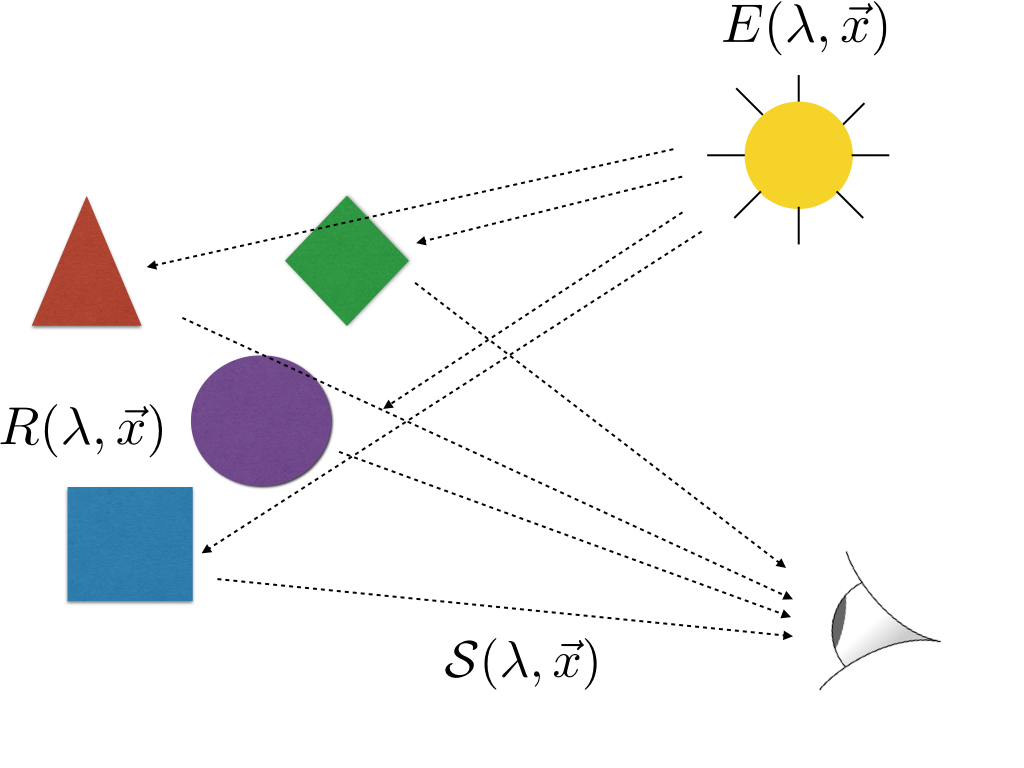
\includegraphics[width=\textwidth]{../FiguresDraft4/Figure1/Figure1_a.png}
        \label{fig:introSchematic}
    \end{subfigure}
    \begin{subfigure}{0.55 \textwidth}   
        \caption{}    
        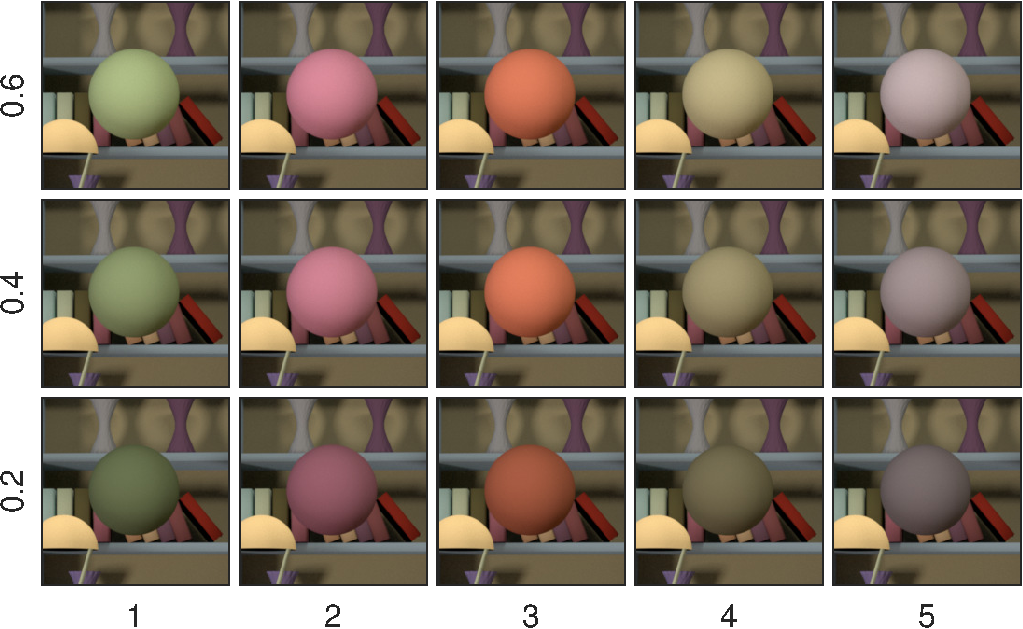
\includegraphics[width=\textwidth]{../FiguresDraft4/Figure1/Figure1_b.pdf}
        \label{fig:introExampleFigure}
    \end{subfigure}
    \label{introFigure}
    \caption{{\bf Color and luminance constancy:} (a)  The light reflected from an object to the eye depends both on the surface reflectance of the object and on the illumination. Additionally, the reflected light also depends on geometric factors, such as the object's shape, pose, and position. The human visual system is able to account for variations in the reflected light due to object-extrinsic factors and produce a percept of object color that is relatively stable across such variations, an ability called color constancy. (b) Images of a sphere under a fixed illuminant.  Down each column, the reflectance function of the sphere varies only by a scale factor; the relative reflectance function is held fixed.  The relative reflectance function (i.e. the shape of the spectral reflectance function) varies across each row.
Within each row, the light reflectance value (LRV) of the spheres is constant. The values on the left of each row provide the corresponding LRV. We cast the problem of computational luminance constancy to be that of estimating the LRV of a target object from the image, across variation in other scene factors. Specifically, we study variation in target object relative surface reflectance, variation in illumination spectrum, and variation in the surface reflectance of the other objects in the scene.}
 \end{figure}

An alternative approach to computational color constancy, which has been less-well explored, is to use supervised machine learning to develop mappings between input images and stable color descriptors \cite{barron2015convolutional}. The use of supervised learning to understand perceptual capabilities for natural stimuli has enjoyed success in domains outside of color vision. For example, a recently developed technique called accuracy maximization analysis (AMA) learns linear filters optimized for particular perceptual tasks \cite{geisler2009optimal}. It has been used to develop ideal observers for speed, focus error, and disparity estimation that provide excellent models of human performance \cite{burge2011optimal, burge2014optimal, burge2015optimal}. In this paper, we apply AMA to a special case of computational color constancy. 

Supervised learning requires large labeled data sets.  Such data sets are not readily available for the study of color constancy. Although there are databases of calibrated color images, these do not provide ground truth information about surface reflectance and illuminantion at each image location \cite{ChakrabartiHyperspectral,NascimentoFoster2016,ParragaHyperspectralData,TkacikUpennHypersepctralData,skauli2013collection,olmos2004biologically}. There are a few databases consisting of images of posed scenes where object surface reflectances are measured individually (\citeNP{funt1988color,ciurea2003large}), but these are not large enough to drive supervised learning.
 
In this paper, we use high-quality computer graphics to generate large data sets of naturalistic images where the surface reflectance corresponding to each image pixel is known. 
This approach allows us to investigate computational color constancy with naturalistic stimuli, while retaining the ability to control the properties of objects and illuminants. More specifically, we use this approach to tackle luminance constancy, a constitutive component of the more general color constancy problem (Fig.~\ref{fig:introExampleFigure}). 

We define the computational problem of luminance constancy as that of estimating the light reflectance value (LRV) of a target object's surface reflectance function.
The LRV is a measure of the overall amount of light reflected by a surface \cite{astm1121477}.
More precisely, the LRV is the luminance of the light that would be reflected to the eye from an object with the 
specified surface reflectance function when the object is illuminated by a reference illuminant,
normalized by the luminance of the reference illuminant itself.
Here we use CIE daylight D65 as the reference illuminant and the CIE 1931 photopic luminosity function to compute luminance \cite{CIE86}.
LRVs range from 0 to 1.

\section*{Methods} \label{Methods}
\subsection{Overview}
There are four key parts to our methods.  First we generate a labeled set of training images.  Second we use a model of the early visual system to compute the responses of the cone photoreceptor mosaic to the labeled images. Third we apply AMA to the cone responses, as well as to a contrast normalized version of the cone responses, to learn task-optimal receptive fields (RFs). Fourth we evaluate how well the responses of the RFs may be decoded to achieve luminance constancy.

\subsection{Labeled training data} \label{method:VirtualWorld}
\subsubsection{Virtual naturalistic scenes}
The light that reflects from objects to the eyes depends on many factors.
These include the surface reflectance, texture, material and geometry of the objects, 
the spectral power distribution function of the illuminants, and the position of the observer.
We have developed a rendering package 
(\href{https://github.com/BrainardLab/VirtualWorldColorConstancy}{https://github.com/BrainardLab/VirtualWorldColorConstancy}) 
that allows us to construct models of naturalistic scenes, with key scene factors under programmatic control.
The package builds on our RenderToolblox4 package (\href{http://rendertoolbox.org}{http://rendertoolbox.org}) \cite{heasly2014rendertoolbox3},
and harnesses the open-source computer graphics renderer Mitsuba (\href{https://www.mitsuba-renderer.org}{https://www.mitsuba-renderer.org}, 
\citeNP{jakob2015mitsuba}) to produce physically-accurate images from the scene models.
Because each image is rendered from a known scene model, each image pixel can be labeled with 
the surface reflectance of the corresponding scene object.
By incorporating statistical models of the variation of object surface reflectance and daylight illumination, 
the pipeline allows us to produce large labeled sets of images that capture key aspects of the task-relevant 
statistical structure of natural scenes.

% Figure 2
\begin{figure}[t]
\centering
\begin{subfigure}[b]{0.22 \textwidth}
        \caption{Library }
        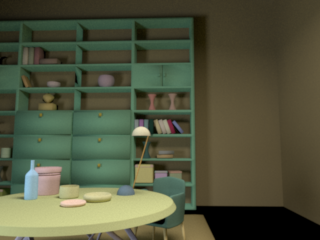
\includegraphics[width=\textwidth]{../FiguresDraft4/Figure3/Figure3_a.png}
        \label{fig:baseSceneLibrary}
    \end{subfigure}
    ~
    \begin{subfigure}[b]{0.22 \textwidth}
        \caption{Mill}    
        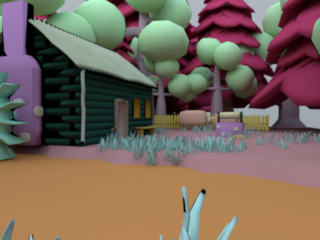
\includegraphics[width=\textwidth]{../FiguresDraft4/Figure3/Figure3_b.png}
        \label{fig:baseSceneMill}
    \end{subfigure}    
    ~
    \begin{subfigure}[b]{0.22 \textwidth}
        \caption{Table-Chairs}    
        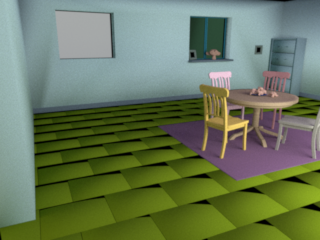
\includegraphics[width=\textwidth]{../FiguresDraft4/Figure3/Figure3_c.png}
        \label{fig:baseSceneTableChairs}
    \end{subfigure}
    \caption{{\bf Base scenes.} Each panel shows a rendering of one base scene without additional inserted objects.  The reflectance spectra of the distinct surfaces and the spectral power distributions of the light sources in each scene have been assigned randomly from models of naturally occurring spectra (see text).}\label{fig:baseScenes}
\end{figure}
%% DHB: We need to think about how to scale the images for display.  The Library scene is too dark, at least when printed.

% Figure 3
\begin{figure}
\centering
    \begin{subfigure}[b]{0.14 \textwidth}
        \caption{Big-ball}
        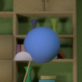
\includegraphics[width=\textwidth]{../FiguresDraft4/Figure4/Figure4_a.png}
        \label{fig:libraryWithBigBall}
    \end{subfigure}
     ~ 
    \begin{subfigure}[b]{0.14 \textwidth}
        \caption{Xylophone}
        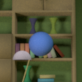
\includegraphics[width=\textwidth]{../FiguresDraft4/Figure4/Figure4_b.png}
        \label{fig:libraryWithXylophone}
    \end{subfigure}
     ~ 
    \begin{subfigure}[b]{0.14 \textwidth}
        \caption{Barrel}
        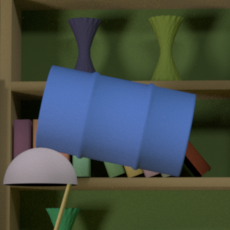
\includegraphics[width=\textwidth]{../FiguresDraft4/Figure4/Figure4_c.png}
        \label{fig:libraryWithBarrel}
         \end{subfigure}
    ~
	\begin{subfigure}[b]{0.14 \textwidth}
        \caption{Ring toy}
        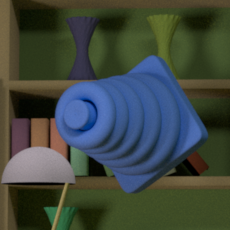
\includegraphics[width=\textwidth]{../FiguresDraft4/Figure4/Figure4_d.png}
        \label{fig:libraryWithRingToy}
    \end{subfigure}
        ~
    	\begin{subfigure}[b]{0.14 \textwidth}
        \caption{Bottle}
        
\includegraphics[width=\textwidth]{../FiguresDraft4/Figure4/Figure4_e.png}
        \label{fig:libraryWithChampagneBottle}
    \end{subfigure}
\caption{{\bf Library base scene with inserted objects.} The rendering package can be used to insert objects into base scenes. The panels show different objects inserted in the library base scene. The objects were inserted at a user defined location in the image. Then the rendering viewpoint was set so that the object is at the center of the rendered image. In these panels, the full rendered image has been cropped so that the inserted object is visually salient.}\label{fig:libraryWithTarget}
\end{figure}
%% DHB: Can we render these examples at higher resolution, so that they look nicer?  The blurriness is distracting in the images.

% Figure 4
\begin{figure}
	\begin{subfigure}[b]{0.18 \textwidth}
    \centering
        \caption{Target position}
        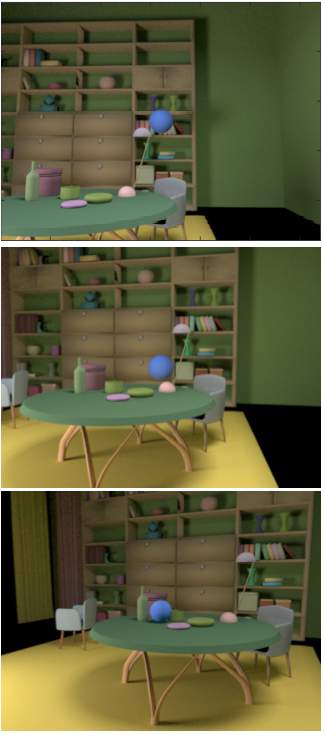
\includegraphics[width=\textwidth]{../FiguresDraft4/Figure5/Figure5_d.png}
        \label{fig:targetPositionVariation}
    \end{subfigure}
    ~
	\begin{subfigure}[b]{0.18 \textwidth}
    \centering
        \caption{Target size/Orientation}
        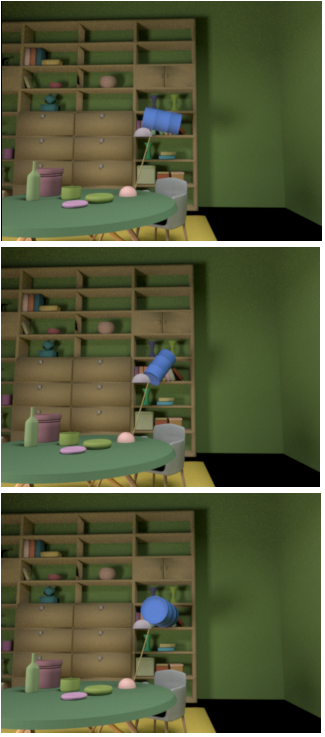
\includegraphics[width=\textwidth]{../FiguresDraft4/Figure5/Figure5_e.png}
        \label{fig:targetSizeOrientation}
    \end{subfigure}
~
\centering
	\begin{subfigure}[b]{0.18 \textwidth}
    \centering
        \caption{Target spectra}
        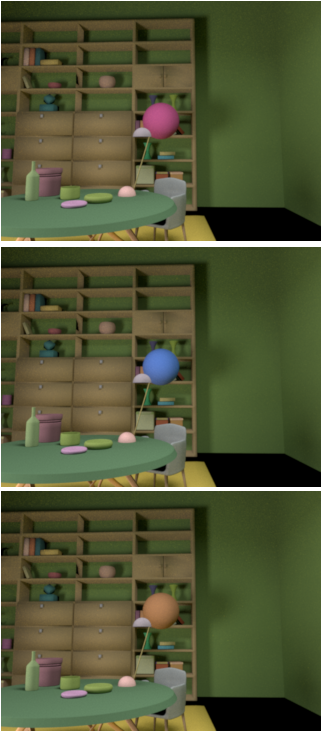
\includegraphics[width=\textwidth]{../FiguresDraft4/Figure5/Figure5_a.png}
        \label{fig:targetVariation}
    \end{subfigure}
    ~
    \begin{subfigure}[b]{0.18 \textwidth}
    \centering
        \caption{Illumination spectra}
        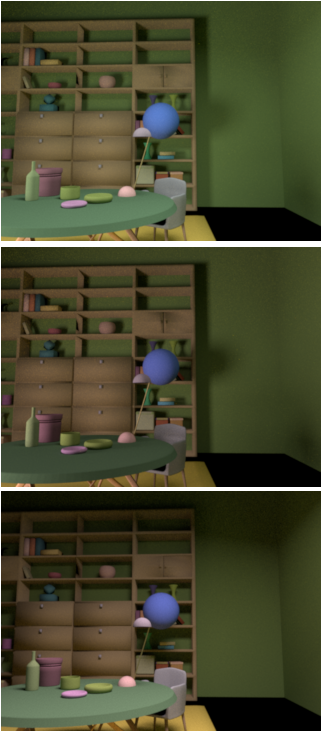
\includegraphics[width=\textwidth]{../FiguresDraft4/Figure5/Figure5_c.png}
        \label{fig:illuminationVariation}
    \end{subfigure}
          ~  
    \begin{subfigure}[b]{0.18 \textwidth}
    \centering
        \caption{Background spectra}
        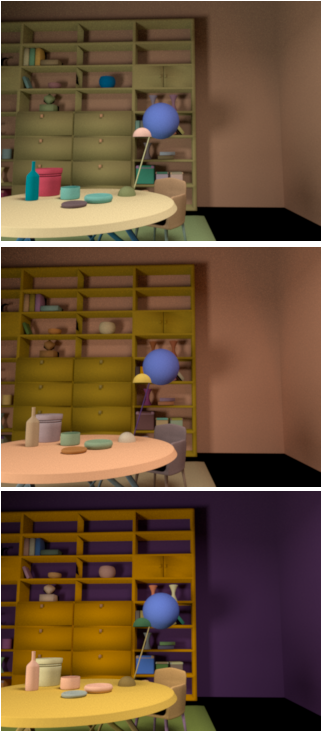
\includegraphics[width=\textwidth]{../FiguresDraft4/Figure5/Figure5_b.png}
        \label{fig:backGroundVariation}
    \end{subfigure}

    \caption{{\bf Scene transformations.} The properties of a visual scene can broadly be classified into two groups: geometrical (a-b) and spectral (c-e). Our rendering package provides control over the properties illustrated by the columns of the figure. (a) Variation in inserted object positions. (b) Variation in object pose. (c) Variation in the surface reflectance of the target object. (d) Variation in the spectral power distributions of the light sources. (e) Variation in surface reflectance of the background objects.
\label{fig:VWCCTransformations}}
\end{figure}
%% DHB: These are too dark in a printout.  Let's review how they are scaled.  Need to make sure we can see an effect of changing the illumination, might want to hand pick the illuminants used here to illustrate the effect.

% Figure 5: Conditions Studied
\begin{figure}
\centering
	\begin{subfigure}[b]{0.33 \textwidth}
		\caption{Condition 1}
%		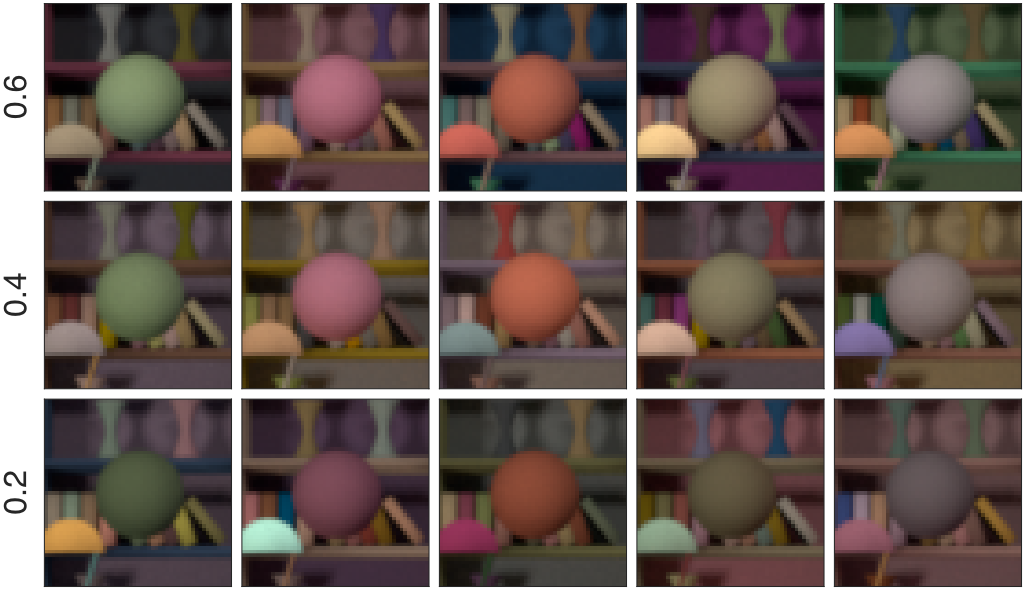
\includegraphics[width=\textwidth]{../FiguresDraft4/Figure2/Figure2_a.png}
		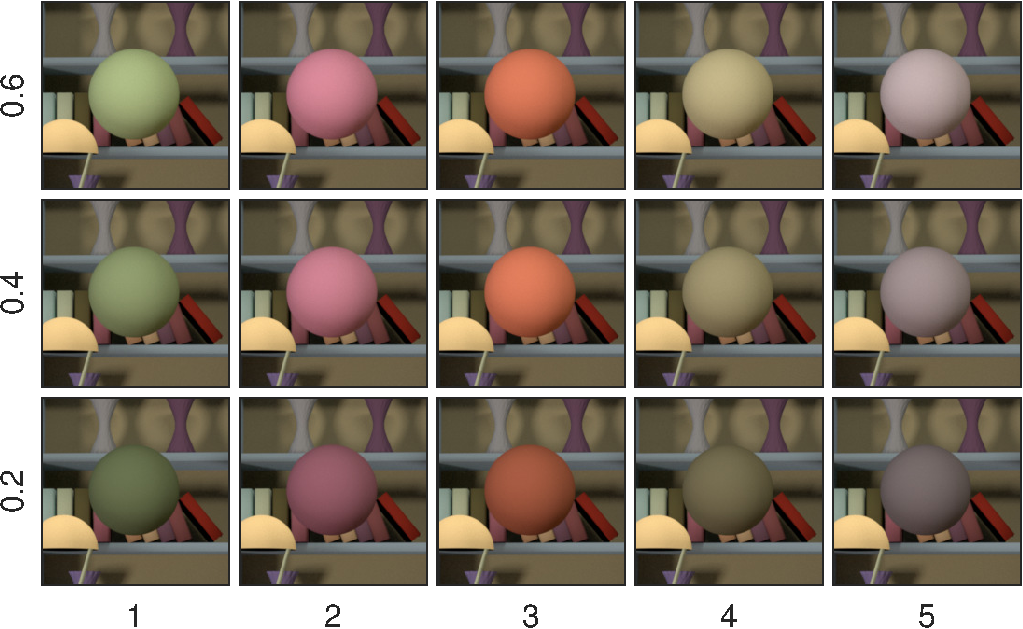
\includegraphics[width=\textwidth]{../FiguresDraft4/Figure1/Figure1_b.pdf}
 		\label{fig:backgroundVarying}
	\end{subfigure}
	\begin{subfigure}[b]{0.33 \textwidth}
        \caption{Condition 2}	
        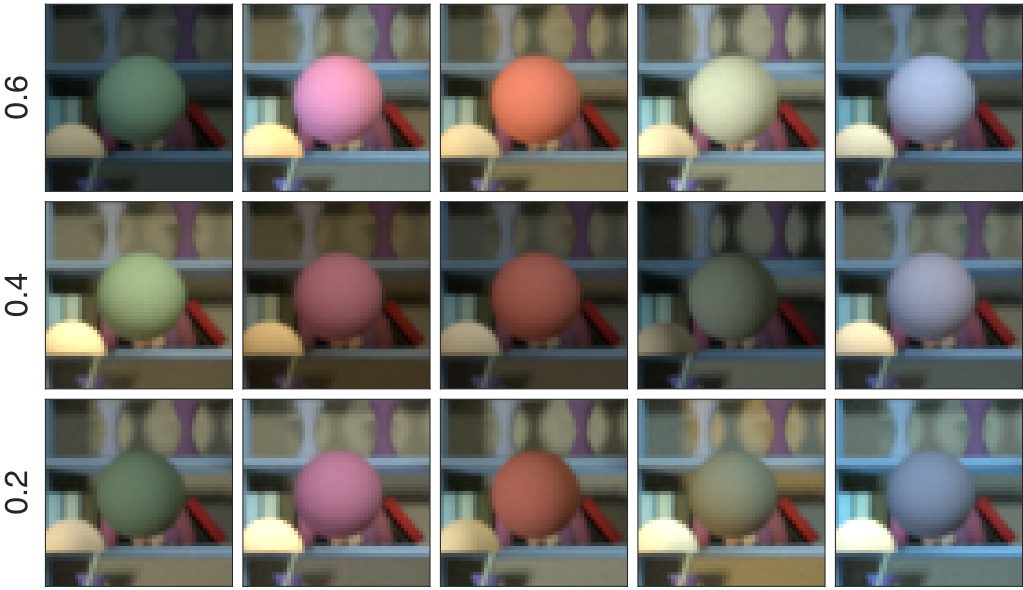
\includegraphics[width=\textwidth]{../FiguresDraft4/Figure2/Figure2_b.png}
        \label{fig:targetIlluminantVarying}
    \end{subfigure}
	\begin{subfigure}[b]{0.33 \textwidth}
	\caption{Condition 3}	
        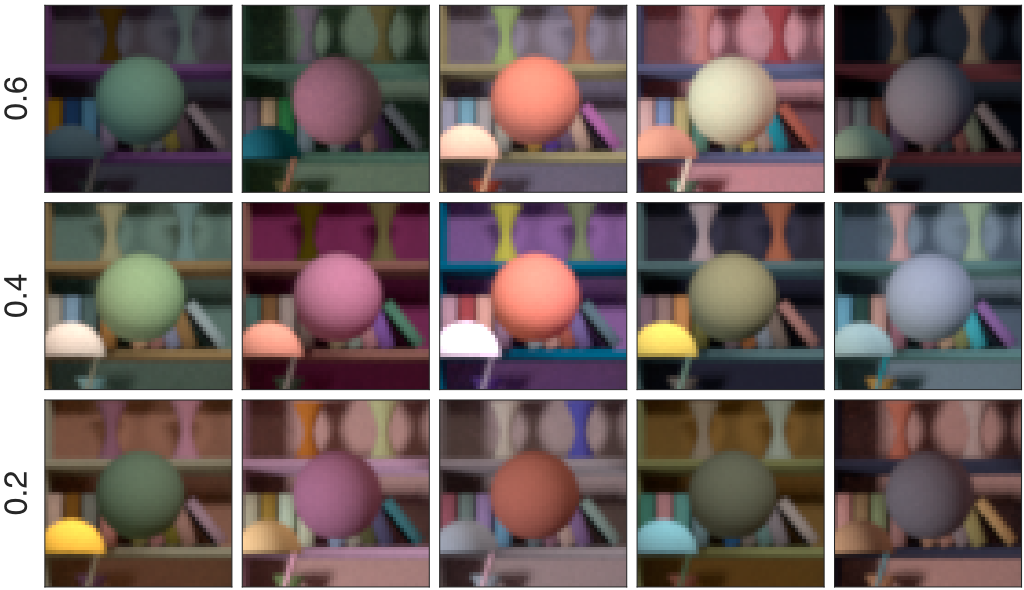
\includegraphics[width=\textwidth]{../FiguresDraft4/Figure2/Figure2_c.png}        
        \label{fig:allSpectraVarying}
    \end{subfigure}    
    \caption{{\bf Dataset Conditions 1-3:} sRGB renderings of illustrative images from the datasets for Conditions 1, 2 and 3. The numbers on the left indicate the standard luminance level of the target object. 5 images are shown at each luminance level. We studied three types of spectral variations. (a) Condition 1: target object relative surface reflectance spectrum variable, light source spectra fixed, background object spectra fixed (same as Fig.~\ref{fig:introExampleFigure}).
(b) Condition 2: target object relative surface reflectance spectrum variable, light source spectra variable, background object spectra fixed, (c) Condition 3: target object relative surface reflectance spectrum variable, light source spectra variable, background object spectra variable. The spheres in each row of each panel have the same surface luminance, while the spheres in each column of each panel have the same relative surface reflectance.  Across the three panels, spheres in corresponding locations have the same surface reflectance. In all three panels, the overall lights source spectra scale factors (see \nameref{Methods}) were drawn from a uniform distribution on the range [0.5, 1.5]. This smaller than the variation we studied, but allows us to show the variation within the dynamic range available for the figure. The sRGB values for all three panels were normalized using a common scale factor prior to gamma correction.} 
\label{fig:studiedCases}
\end{figure}
%% DHB: May also want to render these examples at a higher resolution

Our rendering package includes a collection of base scenes (Fig.~\ref{fig:baseScenes}).
Base scenes specify an arrangement of objects and light sources.
Base scenes may be enriched by the insertion of additional objects, chosen from an object library (Fig.~\ref{fig:libraryWithTarget}).
Once the position, size and pose of the inserted objects has been set, 
our package allows the assignment of a surface reflectance function to each object in the scene 
and a spectral power distribution function to each light source (Fig.~\ref{fig:VWCCTransformations}).
This provides a complete scene model which can be rendered from any specified viewpoint.

In the present work, we used our package to generate datasets of naturalistic scenes and corresponding images.
We used one fixed base scene and inserted a spherical target object of fixed shape and size into this scene.
We generated three distinct datasets, which we refer to as Conditions 1-3 and describe below.
Across these datasets the luminance constancy problem, estimating the target object LRV,
becomes progressively more difficult (Fig.~\ref{fig:studiedCases}).
Each dataset consisted of 1000 scenes and corresponding images.
%% DHB Need to decide how many images we really want for final version of the work.

In Condition 1, we only varied the surface reflectance spectrum of the target object.
The reflectance spectra of the background objects, and the spectral power distributions of the light sources were kept fixed.
In Condition 2, in addition to the reflectance spectrum of the target object,
we also varied the spectral power distribution of the light sources.
Finally, in Condition 3 we varied all three factors (target object surface 
reflectance spectrum, reflectance spectra of the background objects, 
spectral power distribution of the light sources).
We used 10 LRV values, equally spaced between 0.2 and 0.6 and generated 100 target surface reflectance spectra at each of these values. 
The surface reflectance spectra at the same LRV could differ in their relative shape.
The variation within our datasets captures the essence of the computational problem of lightness constancy
up to effects of scene geometry, an additional richness that we do not address in this paper.

For the primary results, we used the ``{\it Library}'' base scene and a spherical target object.
The library base scene contains 2 area lights. 
We inserted one additional spherical spherical light source into the scene.
The position and size of the inserted object, inserted light source and viewpoint were held fixed across all 
scenes in the database. The geometry is shown in Figure~\ref{fig:3DScene}.
Surface and illuminant spectra were drawn according to statistical models of naturally occurring spectra, as described below.
Multispectral images ($320 \times 240$ pixels) were rendered at 31 evenly-spaced wavelengths between $400$nm and $700$nm.
\subsubsection{Illumination spectra}
% Figure 6
\begin{figure}
\centering
    \begin{subfigure}[b]{0.24 \textwidth}
    \centering
	\caption{Granada dataset}
        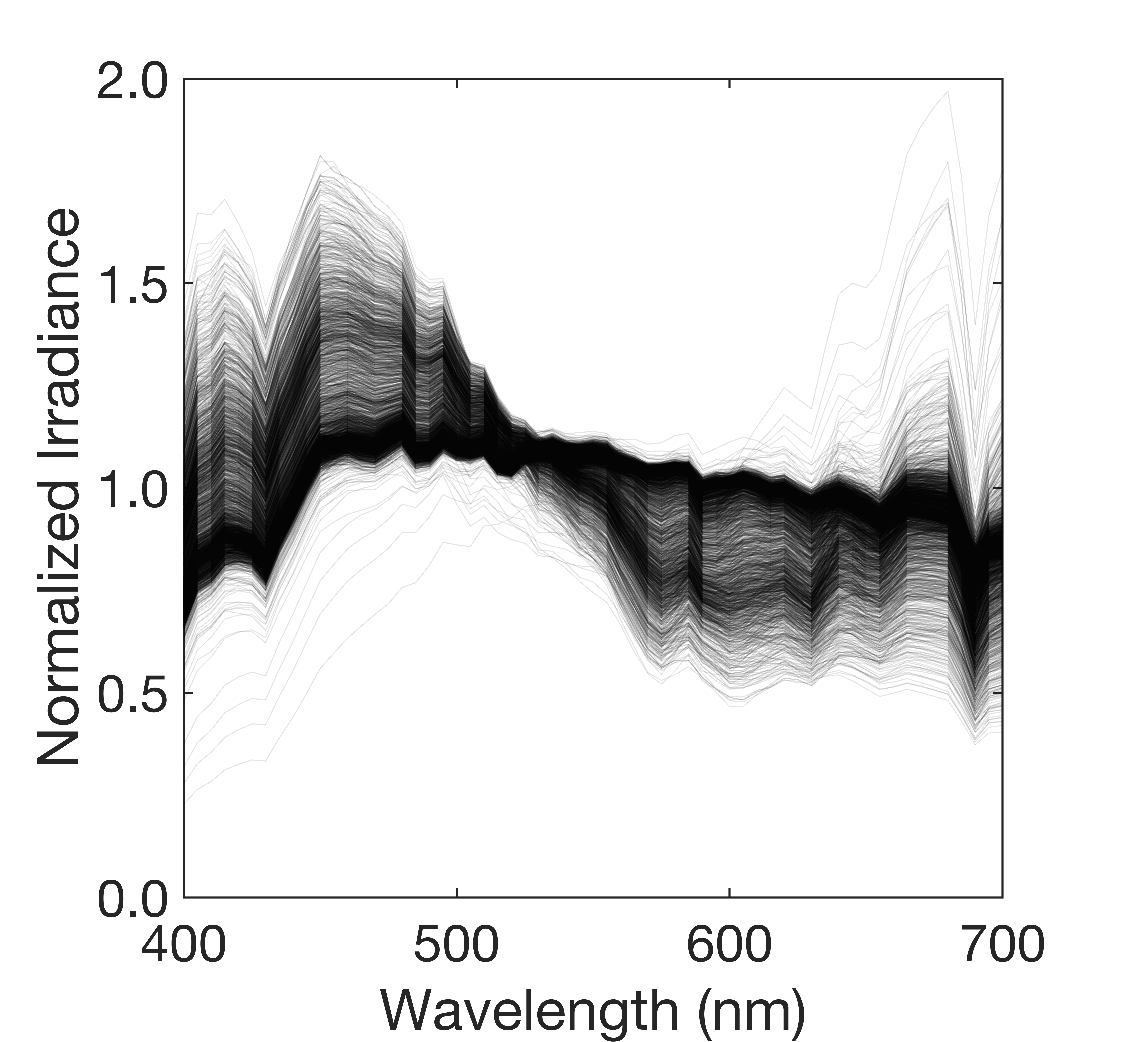
\includegraphics[width=\textwidth]{../FiguresDraft4/Figure6/Figure6_a.pdf}
        \label{fig:granadaData}
    \end{subfigure}
	\begin{subfigure}[b]{0.24 \textwidth}
    \centering
        \caption{Statistical model}
        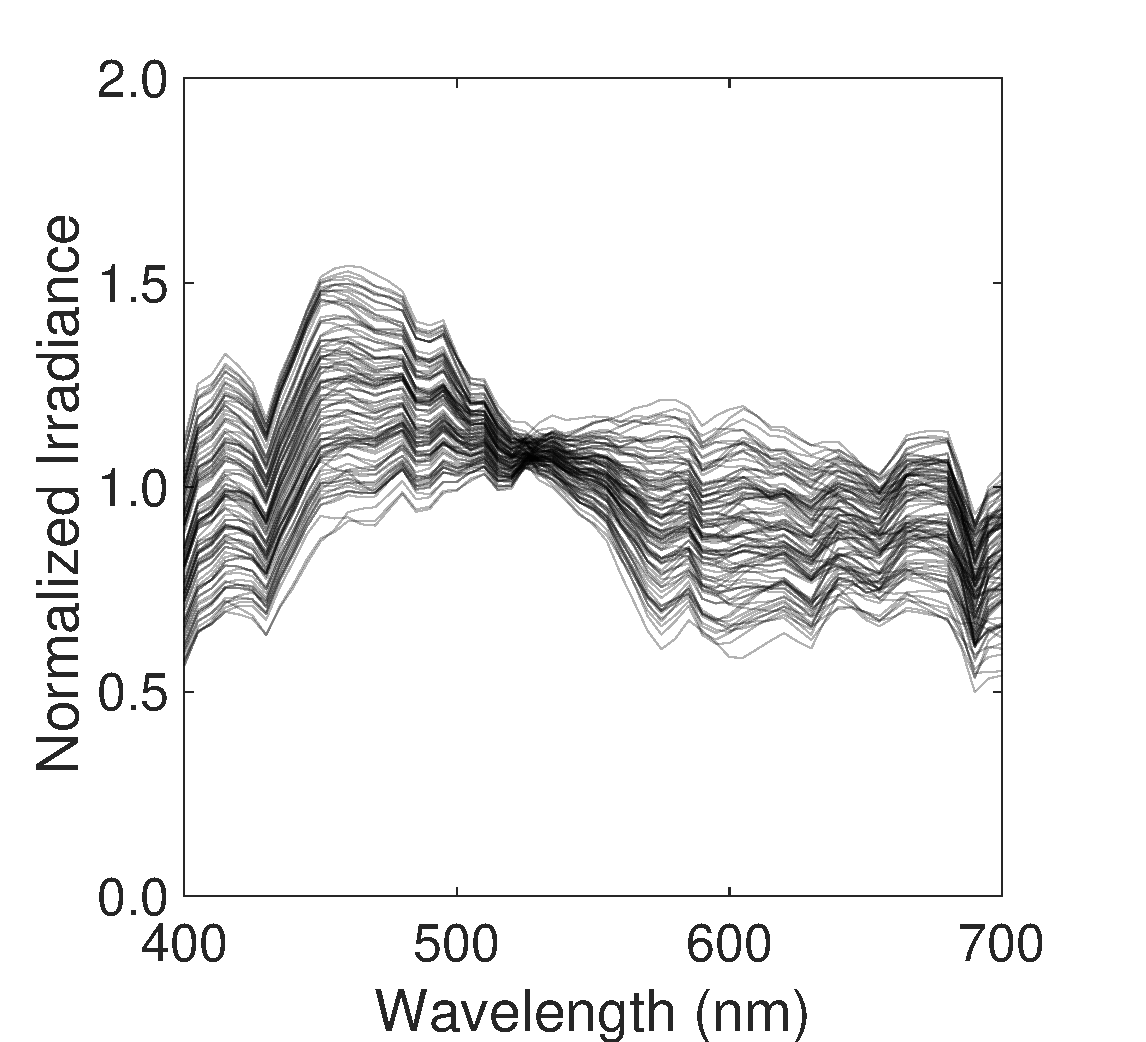
\includegraphics[width=\textwidth]{../FiguresDraft4/Figure6/Figure6_b.pdf}
        \label{fig:illuminantSamples}
    \end{subfigure}
      	\begin{subfigure}[b]{0.24 \textwidth}
    \centering
        \caption{CIE xy chromaticity}
        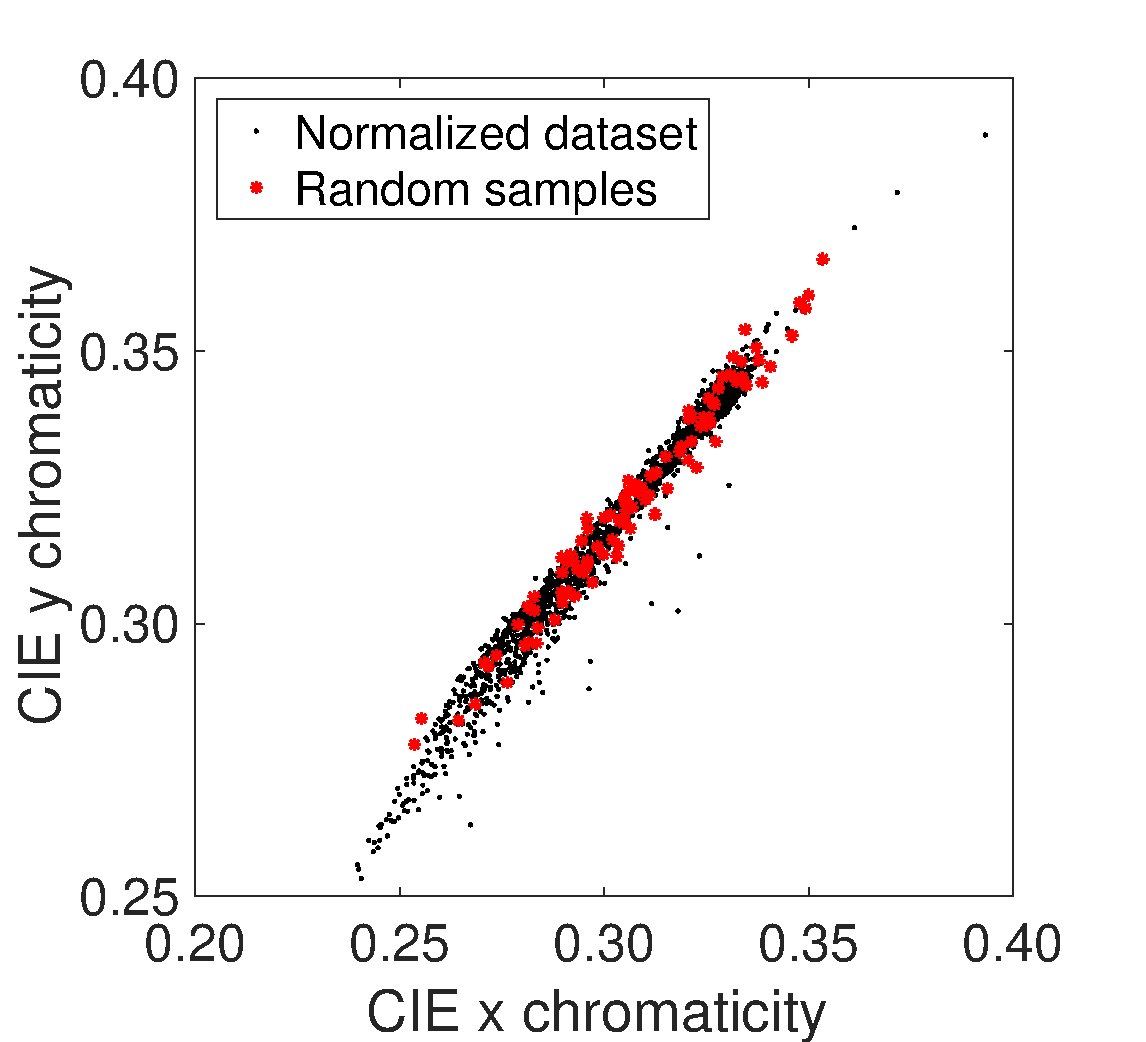
\includegraphics[width=\textwidth]{../FiguresDraft4/Figure6/Figure6_c.pdf}
        \label{fig:xyDiagram}
        \end{subfigure}
      	\begin{subfigure}[b]{0.24 \textwidth}
    \centering
        \caption{Color swatches}
        
\includegraphics[width=\textwidth]{../FiguresDraft4/Figure6/Figure6_d.pdf}
        \label{fig:sRGBIlluminant}
    \end{subfigure}
    \caption{{\bf Statistical model of illumination spectra:} (a) Normalized Granada dataset. Each spectrum is normalized by its mean (with mean taken over wavelength). (b) Sample spectra generated using the statistical model derived from normalized Granada dataset. (c) CIE xy chromaticities of the Granda dataset (black) and the samples shown in b (red). F(d) sRGB renditions of the samples shown in b.}
\label{fig:illuminant}
\end{figure}
%% DHB: The chromaticities in c and renderings in d are for the spectra in b, right?  I wrote the caption to say so, just checking.
%% VS: Yes

To generate illumination spectra, we developed a statistical model of the Granda daylight measurements (\citeNP{hernandez2001color}, \href{http://colorimaginglab.ugr.es/pages/Data}{http://colorimaginglab.ugr.es/pages/Data}) and sampled randomly from the model (see appendix).
The overall intensity of the measurements spans approximately three orders of magnitude.
Figure~\ref{fig:granadaData} plots the measurements in normalized form to make apparent the variation in the relative spectra.

Our statistical model approximates the normalized Granda spectra using their first 6 principle components.
The variation in these components is modeled with a 6-dimensional Gaussian whose mean and covariance matrix 
match the sample mean and covariance of the weights on these components obtained from the normalized Granada spectra \cite{BrainardFreeman}.
To generate a random relative illuminant spectrum, we take a draw from this Gaussian to obtain weights and then use the weights to generate the corresponding spectrum.
Figure~\ref{fig:illuminantSamples} illustrates the relative spectra of draws obtained using this procedure.
Details of the statistical model for illumination are provided in the appendix.
Chromaticities and rendered color renditions of these draws are shown in Figures~\ref{fig:xyDiagram} and ~\ref{fig:sRGBIlluminant}.

Because our multivariate Gaussian model is based on normalized spectra, it does not embody the large variation in overall intensity of natural daylights.
To obtain illuminant spectra with intensity variation similar to the Granada dataset, we scaled each randomly generated relative spectrum.
The scale factors were sampled randomly on a log-uniform scale in the range [0.15, 150].
%% DHB: Check that these values are right.  Linear spacing or log spacing?
%% VS: Yes, log spacing, I have updated the text.

\subsubsection{Surface reflectance spectra}
% Figure 7 Surface Reflectance Data and Model
\begin{figure}
\centering
	\begin{subfigure}{0.24 \textwidth}
    \centering
            \caption{Munsell and Vrhel dataset}
        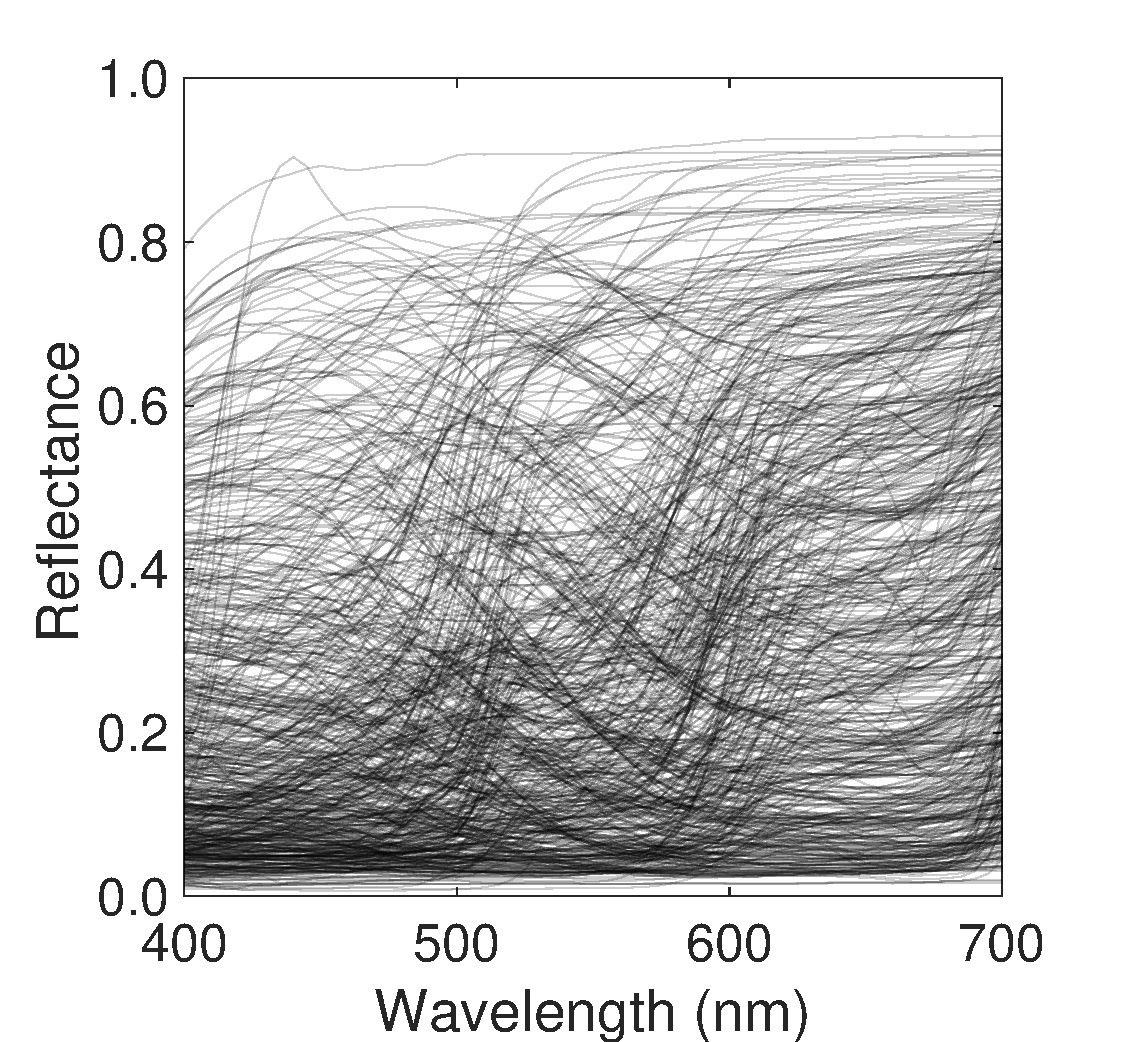
\includegraphics[width=\textwidth]{../FiguresDraft4/Figure7/Figure7_a.pdf}
        \label{fig:reflectanceSpectra}
    \end{subfigure}
    \begin{subfigure}{0.24 \textwidth}
    \centering
        \caption{Statistical model}
        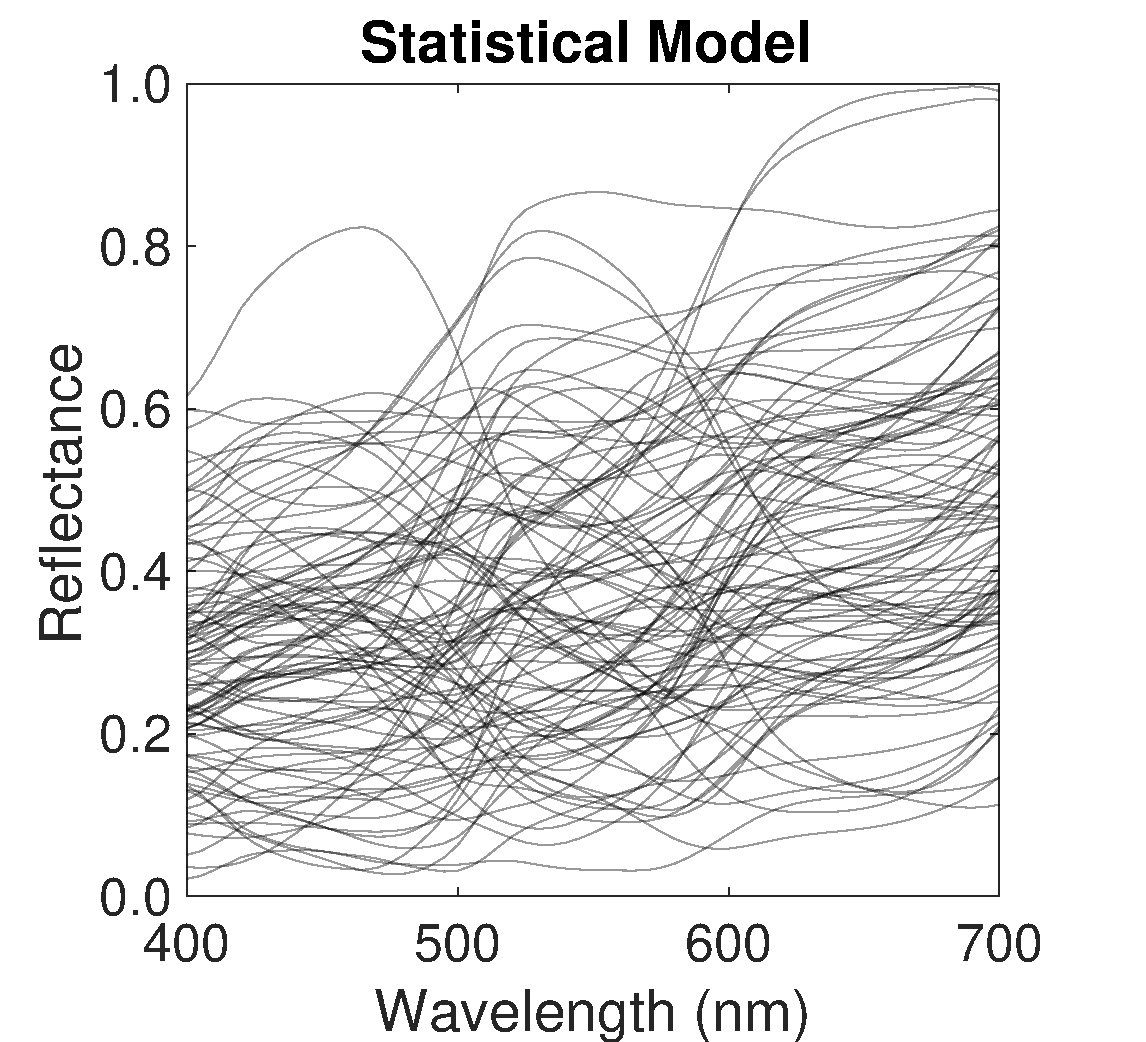
\includegraphics[width=\textwidth]{../FiguresDraft4/Figure7/Figure7_b.pdf}
        \label{fig:reflectanceSamples}
    \end{subfigure}
    \begin{subfigure}{0.24 \textwidth}
    \centering
    \caption{CIE xy chromaticity}
        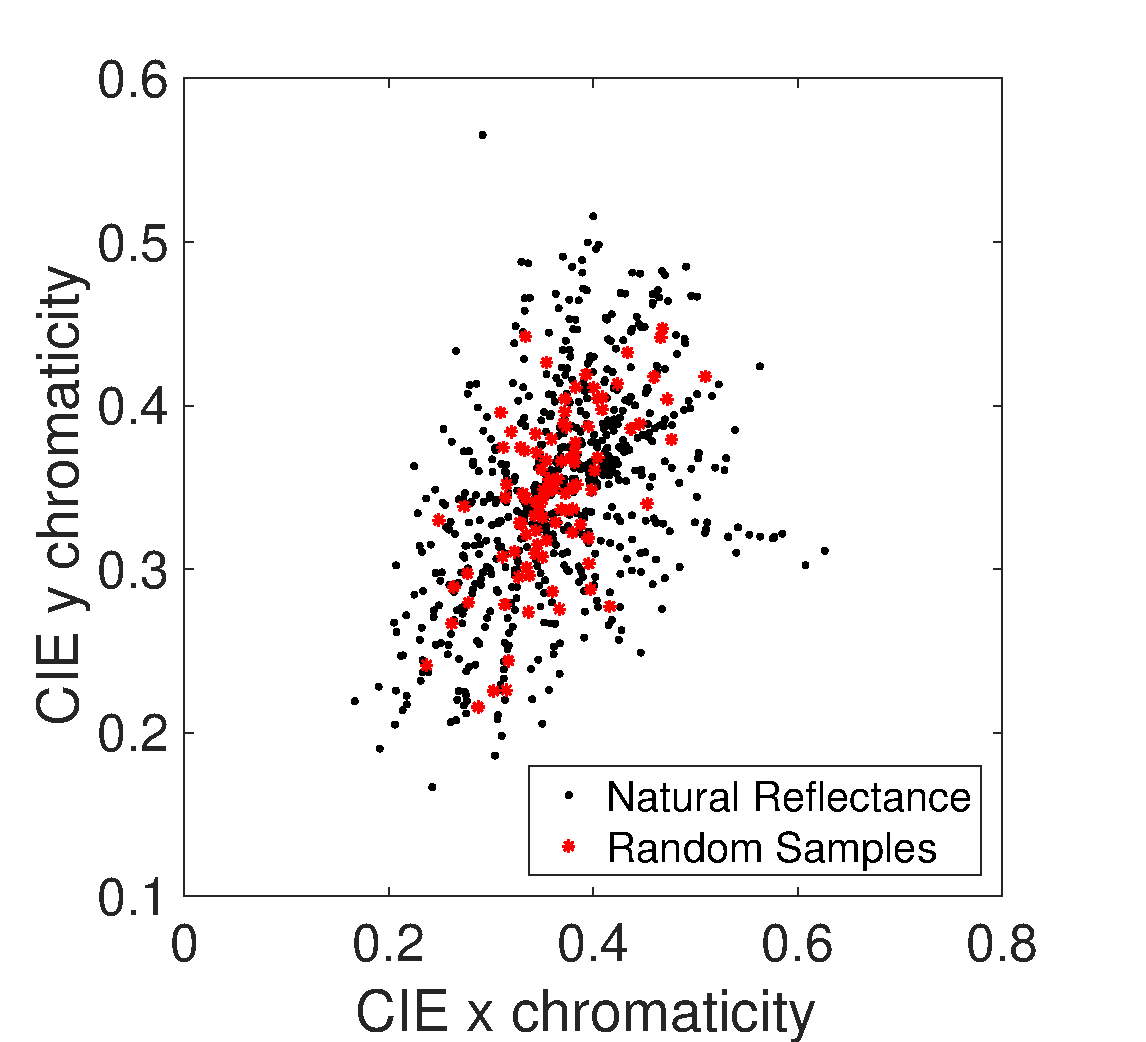
\includegraphics[width=\textwidth]{../FiguresDraft4/Figure7/Figure7_c.pdf}
        \label{fig:xyChroReflectance}
    \end{subfigure}    
    \centering
	\begin{subfigure}{0.24 \textwidth}
    \centering
        \caption{Color swatches}
        
\includegraphics[width=\textwidth]{../FiguresDraft4/Figure7/Figure7_d.pdf}
        \label{fig:backgroundSwatches}
    \end{subfigure}
    \caption{{\bf Statistical model of surface reflectance:} (a) Surface reflectance spectra from the Munsell and Vrhel datasets. (b) Sample spectra generated using the surface reflectance statistical model. (c) CIE xy chromaticity diagram of the Munsell and Vrhel reflectances and samples shown in b (red). (d) sRGB renditions of the samples shown in b, rendered under the CIE D65 daylight.}
\label{fig:surfaceReflectanceGeneration}
\end{figure}
%% DHB: The chromaticities in c and renderings in d are for the spectra in b, right?  I wrote the caption to say so, just checking.
%% VS: Yes

%Figure 8 Target Surface Reflectance Samples
\begin{figure}
\centering
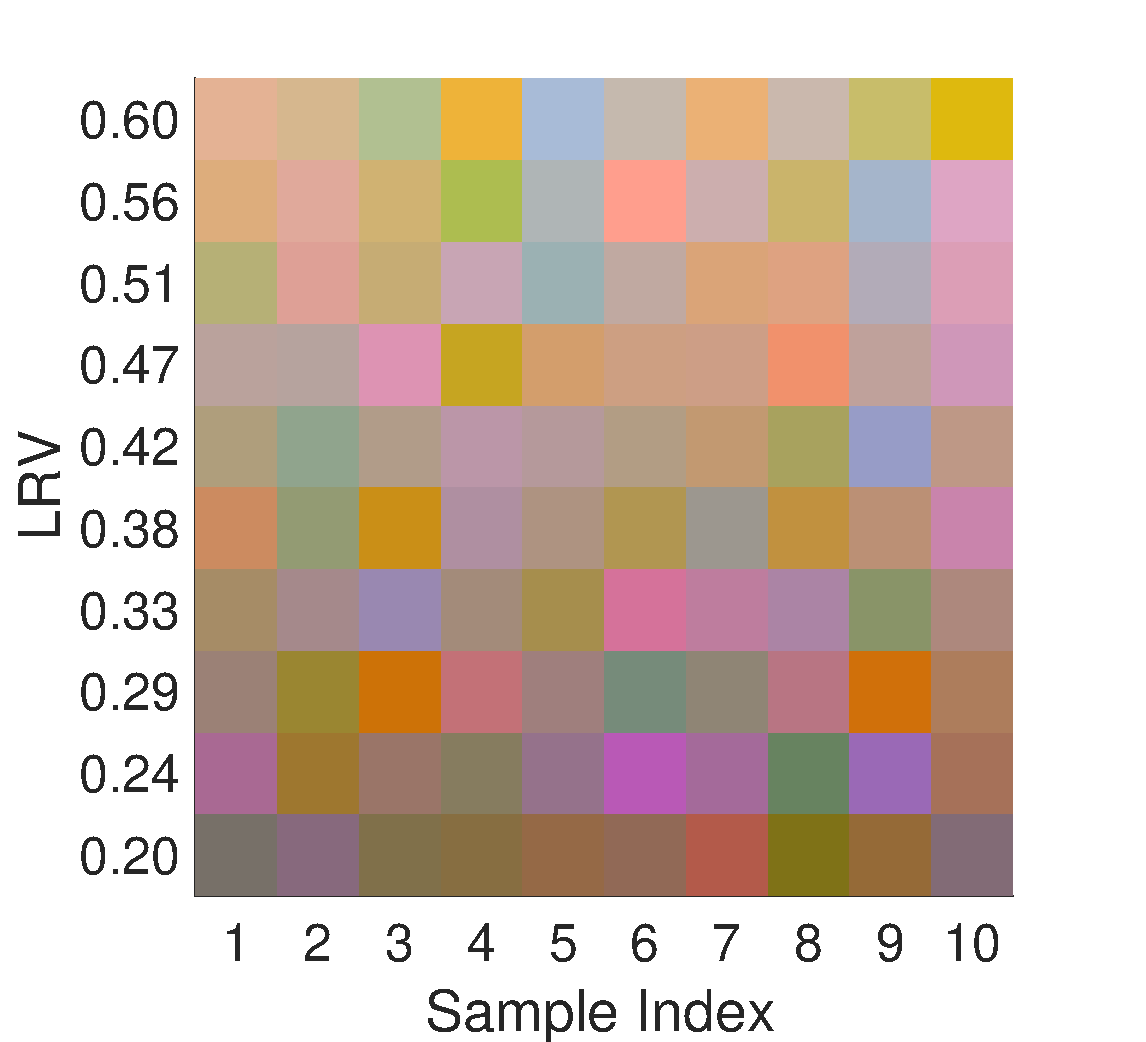
\includegraphics[width=0.3\textwidth]{../FiguresDraft4/Figure8/Figure8.pdf}
\caption{{\bf Target object surface reflectance spectra:} sRGB renditions of the target object surface reflectance rendered under CIE D65 daylight spectrum. The figure shows 10 random samples at 10 equally spaced LRV levels in the range [0.2, 0.6]. Each row contains 10 random samples of reflectance spectra generated at the LRV shown on the left.}
\label{fig:targetSwatches}
\end{figure}

We generated random reflectance spectra using the same principles we used to model illuminant spectral power distributions.
We combined the Munsell \cite{kelly1943tristimulus} and Vrhel \cite{vrhel1994measurement} surface reflectance 
measurements to create a database containing 632 reflectance spectra (Figure~\ref{fig:reflectanceSpectra}).
The Munsell database contains 462 spectra each measured at 5 nm sampling intervals between 380nm and 780nm.
The Vrhel dataset contains 170 spectra measured at 2 nm sampling between 390 nm and 730 nm.
We resampled these spectra to 31 evenly-spaced wavelengths between 400 nm and 700 nm (Figure~\ref{fig:reflectanceSpectra}).
Details of the statistical model for surface reflectance spectra are provided in the appendix. 
Figures~\ref{fig:reflectanceSamples},~\ref{fig:xyChroReflectance}, and~\ref{fig:backgroundSwatches} illustrate reflectance draws obtained using the model. 

For generating the target object reflectance at a particular luminance, the values in a generated spectrum were 
scaled such that the LRV had the desired value (see appendix).
Figure \ref{fig:targetSwatches} shows color renderings of target reflectance spectra under CIE illuminant D65, for the evenly spaced LRV values we studied.
%% DHB: Note that this procedure is different than conditioning the statistical model on the target LRV.  We could switch to the latter if we wished.
%% VS: I don't think it matters if we care about keeping only one color co-ordinate fixed.

% Figure 8: Methods
\begin{figure}
\centering
\begin{subfigure}[b]{0.25 \textwidth}
		\centering
        \caption{sRGB rendering of a 3D scene}
        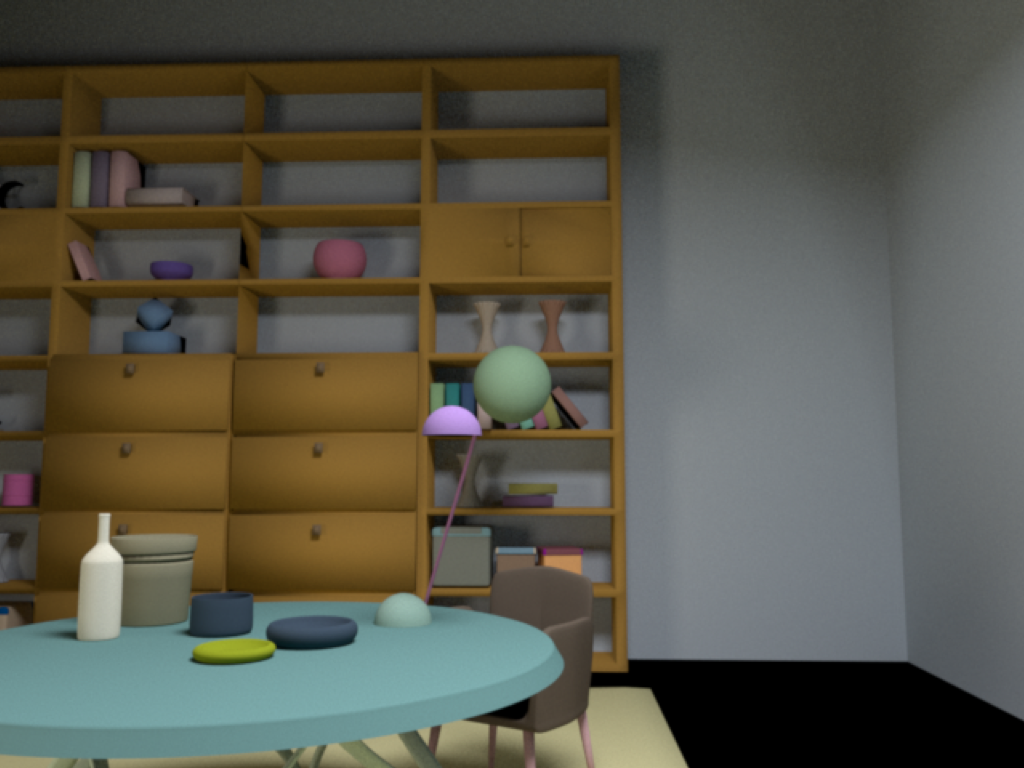
\includegraphics[width=\textwidth]{../FiguresDraft4/Figure9/Figure9_a.png}
        \label{fig:3DScene}
    \end{subfigure}
    ~ 
    \begin{subfigure}[b]{0.19 \textwidth}   
    \hspace{0.1 \textwidth}
        \caption{Cropped image}
        \vspace{1.5mm}
        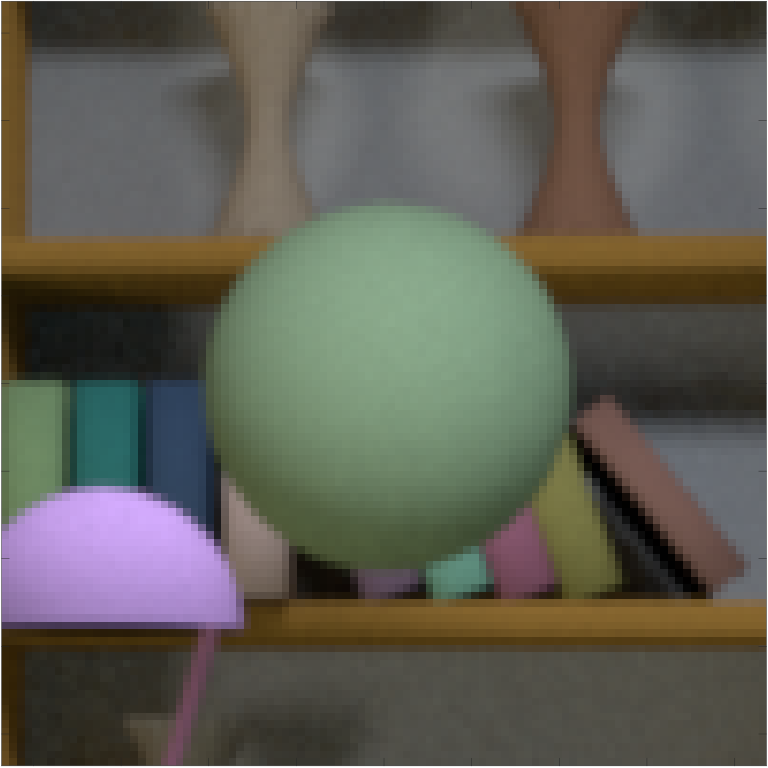
\includegraphics[width=\textwidth]{../FiguresDraft4/Figure9/Figure9_b.png}
        \label{fig:croppedImage}
    \end{subfigure}
    ~ 
    \begin{subfigure}[b]{0.19 \textwidth}
    \hspace{0.1 \textwidth}
        \caption{Retinal image}
        \vspace{1.5mm}
        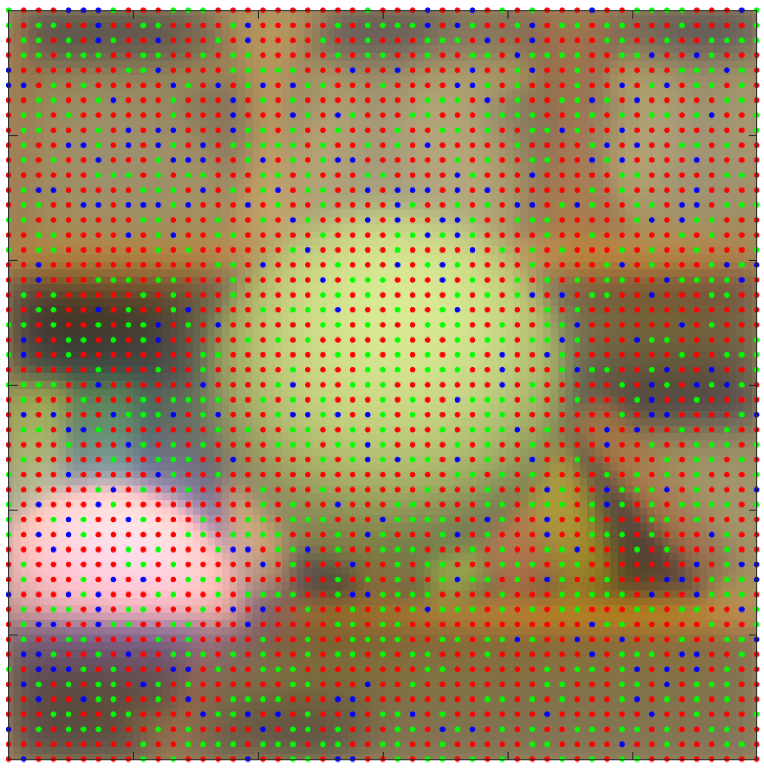
\includegraphics[width=\textwidth]{../FiguresDraft4/Figure9/Figure9_c.png}
        \label{fig:croppedImageWithMosaic}
    \end{subfigure}
    ~
    \begin{subfigure}[b]{0.2 \textwidth}
        \caption{LMS normalized cone contrast}
        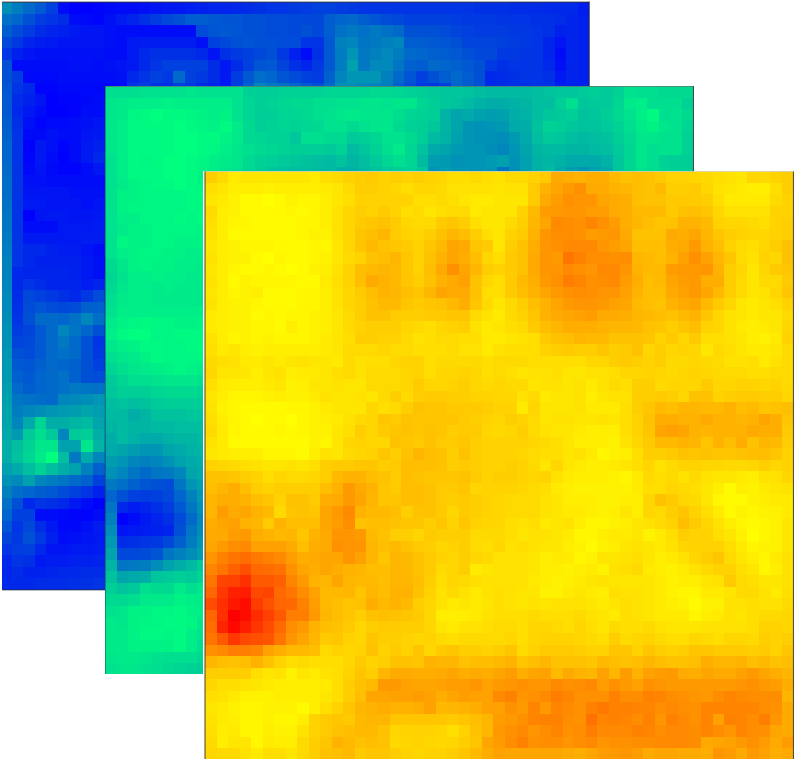
\includegraphics[width=\textwidth]{../FiguresDraft4/Figure9/Figure9_d.png}
        \label{fig:coneContrast}
    \end{subfigure}
    \label{fig:sceneWithCroppedImage}
    \caption{{\bf Pipeline for generating labeled datasets:}  For the supervised learning approach employed in this work, labeled images are generated as follows: (a) A 3D virtual scene, containing a target object is created. The rendering viewpoint is selected so that the target object is in the center of the image. Spectra are assigned to the target object, illuminants, and other objects in the scene using the statistical models described in the text. A multispectral image of the scene is then rendered. (b) The central portion of the rendered image, which contains the target object, is cropped. (c) The retinal image corresponding to the rendered image is computed, and this is used in turn to compute the excitations (taken as the number of photopigment isomerizations) of the cone photoreceptors. The figure shows the a rendering of the retinal image after optical blurring, with the location and identity of the cones indicated by an overlay (L cones: red, M cones: green, S cones: blue).  (d) The cone excitations are interpolated to estimate the responses of all the three types of cone at each location (demosaicing). Finally, the demosaiced images are contrast normalized separately for each cone type.}
\end{figure}

\subsection{Model of early visual system} \label{method:Isetbio}
The light entering the eye is blurred by the eye's optics.
The resulting retinal image is sampled by a mosaic of cone photoreceptors.
The excitations of these photoreceptors provide the information about the scene that is available to the neural visual system for further processing.
Because we are interested in how well luminance constancy may be achieved by the human visual system, we simulated the cone excitations
to our scenes using a model of the early visual system.

We focussed our analysis on regions of the image local to the target by cropping the rendered images to $1 \times 1$ degrees of visual angle around the target object ($51 \times 51$ pixels; Figure~\ref{fig:croppedImage}).
This choice is motivated by the observation that neural receptive fields in the early visual pathways (e.g., retina, primary visual cortex) pool information locally.
In foveal primary visual cortex, receptive fields have a spatial extent of approximately 1 degree of visual angle (REFS).
%% DHB: Johannes to provide his favorite citation or two.  Some review.

We modeled a visual system with a pupil diameter of 3 mm, optical blurring (including axial chromatic aberration) in the formation of the retinal image \cite{marimont1994matching}, and spatial sampling by an interleaved mosaic of long (L), middle (M)  and short (S) wavelength-sensitive cones (\citeNP{brainard2015color}; Fig.~\ref{fig:croppedImageWithMosaic}). 
The cone mosaic contained L:M:S cones in the ratio 0.6:0.3:0.1 and with spectral sensitivities derived from the CIE physiological standard \cite{CIE86}.
Cone excitations were taken as the number of photopigment isomerizations, assuming an integration time of 100 msec, and we modeled the Poisson nature of photopigment isomerization \cite{hecht1942energy}. 
This modeling was implemented using the software infrastructure provided by ISETBio (\href{https://isetbio.org}{https://isetbio.org}).

%% Details on ISETBIO computations from Nicolas (TEXT IN CAPS IS FROM VIJAY)
%% Scene: 
%%- the default mean luminance was set to 200, but there is a key-value param that could have overriden this value. 
%%  I do not know if this were the case.
%%
%% % MEAN LUMINANCE = 0, NO SCALING
%
%%- The default FOV was 1 deg, but there is a key-value param that could have overriden this value.
%%  I do not know if this were the case.
%%
%% % HORIZONTAL FOV = 1
%%
%%- Distance default is 1 meter, but there is  a key-value param that could have overriden this value.
%%  I do not know if this were the case.
%%
%%% DISTANCE 1M
%%
%%Optics: 
%%- 3 mm pupil, 17 mm focal length, with a spectro-spatial OTF described in  
%%  (Marimont & Wandell (1994) J. Opt. Soc. Amer. A,  v. 11, p. 3113-3122), 
%%   which includes axial chromatic aberration. However, there is key-value param o skip the OTF. 
%%   Not sure if this was used.  It it was used, the optics was set to diffraction limited.
%%
%% % SKIP OTF OFF:  'skipOTF', false ...  
%%
%%Lens: 
%%- not sure if the optical density is from Wyszecki&Stiles or from Stockman-Sharpe. 
%%  The isetbio file commend only says it is from PTB. David do you know, or should I check
%%  the data?
%%
%%Cone Mosaic: 
%%- rectangular cone mosaic with 0.6:0.3:0.1 LMS densities
%%- FOV was a key-value param, so I do not know what was used.
%%- Also the mosaic was subsampled  according to a cone-stride param, with a default of 15 cones
%%but there is a key-value param that could have overriden this value. I do not know what that parameter value was.
%%
%% CONE STRIDE = 3 'coneStride', 3, ... 
%%
%%
%%- There is a key-value pair to also low-pass the optical image with default value to not do so.
%%  If that was user-overriden the OI was lowpass filtered using a Gaussian whose sigma was dependent on the cone-stride param.
%%
%% LOW PASS FILTER = MATCH CONE STRIDE : lowPassFilter = 'matchConeStride';      
%%
%%- IntegrationTime was not specified, so it was the default which is 5 msec.
%%  The cone isomerization maps were also demosaiced using linear interpolation.
%%- The default isomerization noise was set to none, but there is a key-value parameter
%%  that can override it. I do not know what the value of that was.
%%
%% ISOMERIZATION NOISE = FROZEN, 'isomerizationNoise', 'frozen'
%%
%%-  Finally, there is a key-value param named 'coneEfficiencyBasedReponseScaling', which by default is set to 'none'
%%   But if it was user-set to non 'none' the code scaled the responses to simulate equal quantal efficiencies 
%%   for L , M and S coneEfficiencyBasedReponseScaling by undoing filtering by the lens and the macular pigment.
%%   I do not know if this was used.
%% 
%% coneEfficiencyBasedReponseScaling = 'area'

The cone excitations represent the first step of visual processing.
To capture key properties of post-receptoral processing, such as contrast normalization \cite{heeger1992normalization,albrecht1991motion,carandini2012normalization},
we processed the excitations as follows:
First, we generated a response for each cone class at each pixel in the sampled retinal image, using linear interpolation separately for each cone class.
This gives us a cone excitation image for each cone class.
We also normalized each cone excitation image by the total area under the corresponding cone spectral sensitivity.
This makes the magnitude of the cone excitation images similar across cone classes.
These two processing steps do not alter the information in the cone excitation images. 

To model contrast coding, we converted each cone excitation image to a corresponding cone contrast image.
This was accomplished by computing the mean response over the three cone excitation images, and then subtracting off and dividing by this mean.
To model contrast normalization, we divided the contrast images by the sum of squared contrasts taken over image pixels and cone classes.

%% DHB: We meed to figure out and say something about how we scaled image intensities into a reasonable range.

\subsection{Computational luminance constancy} \label{method:SupervisedLearning}
We used our datasets to determine how well target object LRV can be estimated from cone excitations and from normalized cone contrasts.
Studying both representations allows us to understand how early contrast coding and normalization affect how well luminance constancy can be achieved.
We applied accuracy maximization analysis (AMA) to learn the optimal receptive fields for estimating LRV,
and evaluated the performance obtained when the output of these filters was optimally decoded.

\subsubsection*{Learning optimal filters}
AMA is a task specific Bayesian method for dimensionality reduction.
When provided with a labeled training set, a receptive field response model, a decoder that uses these responses to estimate the stimulus label, and a cost function, AMA returns a set of linear receptive fields.
Given a set of linear receptive fields and an explicit cost function, it is possible to determine the minimum-expected-cost estimator that maps responses to stimulus labels given the training set and the 
assumption that all images in the training set are equally likely.
Moreover, the corresponding expected estimation cost may be explicitly computed.
AMA searches over the space of linear receptive fields to find the set that minimizes the expected estimation cost.
Here we used squared error as the cost function and assumed that receptive field responses were corrupted by scaled Gaussian noise (i.e. Poisson-like noise with a fano factor of 1.3).
Details of how AMA learns filters and the filter responses are optimally decoded are provided in previously published work \cite{geisler2009optimal,burge2017accuracy,jaini2017linking}.

\subsubsection*{Decoding optimal filters}

Once the optimal receptive fields have been learned, we need to develop a general decoder that can be applied to arbitrary test stimuli.
A general decoder is necessary because the decoder used to learn the receptive fields requires the response mean and response variance of the filters to every labelled stimulus in the training set \cite{geisler2009optimal,burge2017accuracy}.
To proceed, first we use the AMA optimal receptive fields and the training dataset to find the conditional distributions of the receptive field responses, conditioned on the labelled target object LRVs.
Then, we approximate these with multivariate Gaussian distributions.
To estimate the LRV of the target object in a test image, we use Bayes' rule together with the Gaussian conditional distributions and a uniform prior to obtain the posterior distribution over LRV values given the filter responses.
The optimal estimate is the LRV value that minimizes the expected value of the cost function, where the expectation is taken over the posterior.
Here we use a Kullback-Leibler divergence cost function, so that the optimal estimator is the maximum a posteriori estimate.
%% DHB: Uniform prior, right? And posterior mean?  If not, correct prose above.

\subsubsection*{Baseline methods}

To provide baselines for evaluation of the estimation method described above, we used linear regression.
First, we solved for the weights on the average L, M and S cone excitations corresponding to the target object that best predicted the target LRV values.
We took the average cone responses from a $3 \times 3$ region at the center of the target object.
This baseline method disregards information carried the image regions corresponding to the background objects.
We also performed regression on the contrast normalized version of the cone responses.
This second baseline method indirectly incorporates information carried in the image regions corresponding to the background objects,
through their effect on the contrast normalized responses at the center of the target object. 
We also evaluated the performance of a naive model that estimates the mean of the LRV values in the training set, irrespective
of the image data.

\section{Results} \label{Results}
%% Figure 10: Results for Condition 1
\begin{figure}
\centering
            \begin{subfigure}[b]{0.25 \textwidth}
        \caption{LRV estimates}
        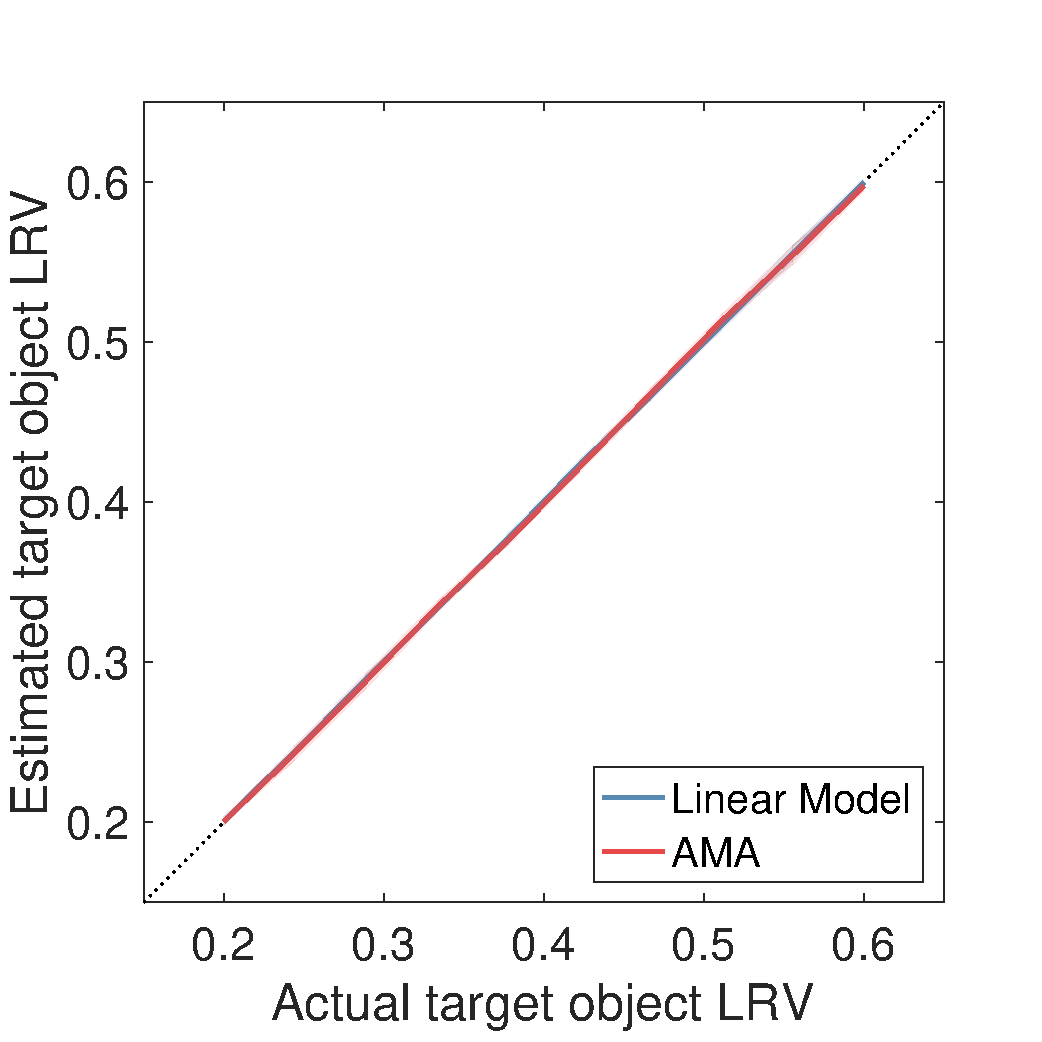
\includegraphics[width=\textwidth, trim={0 0 0 1.3cm},clip]{../FiguresDraft4/Figure10/Figure10_a.pdf}
        \label{fig:case1Estimates}
    \end{subfigure} 
        \begin{subfigure}[b]{0.26 \textwidth}
        \caption{RF responses}
        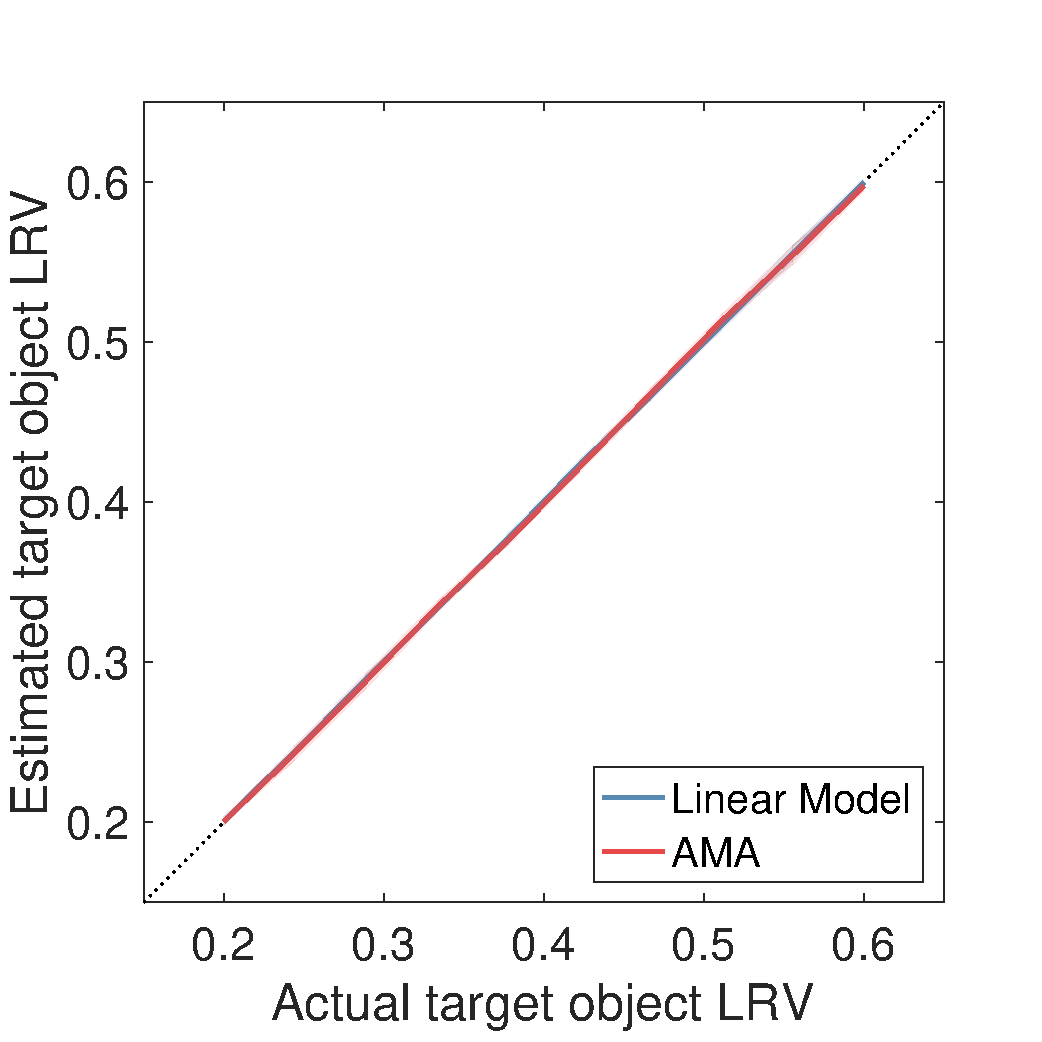
\includegraphics[width=\textwidth, trim={0 3mm 0 15mm},clip]{../FiguresDraft4/Figure10/Figure10_b.pdf}
        \label{fig:case1RFResponse}
    \end{subfigure}
    \begin{subfigure}[b]{0.4 \textwidth}
	\caption{AMA receptive fields}
	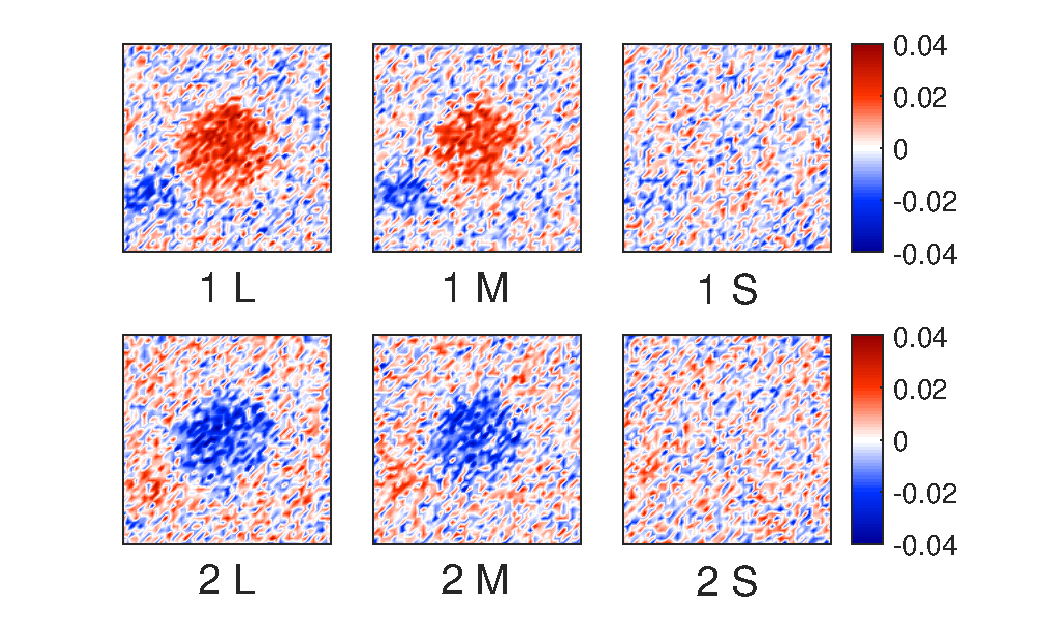
\includegraphics[width=1.0\textwidth, trim={0.2cm -0.cm 0 0.3cm}]{../FiguresDraft4/Figure10/Figure10_c.pdf}
	\label{fig:case1RFs}
    \end{subfigure}   
    \caption{{\bf Condition 1 results:} (a) Mean estimated LRV $\pm$ 1 standard deviation for images in the test set obtained using linear regression and AMA estimators, based on the cone excitations. Solid lines show the mean estimate, the filled region in lighter color shows $\pm$ 1 standard deviation. The diagonal identity line (dotted blue) indicates veridical estimation. The standard deviations are too small to be visible. Relative RMSE (see Fig.\ref{fig:barGraphs}) is 0.8\% for linear regression and 1.1\%  for AMA based estimation. (b) Cone excitations projected along the first two AMA receptive fields for training images of Condition 1. Each cloud represents the image patches corresponding to one LRV. The clouds are approximated by a multivariate Gaussians whose means and variances are approximated by the ellipses shown in the figure. (c) The first two AMA receptive fields learnt using the cone excitations of stimuli in the training set.}
\label{fig:Condition1}
\end{figure}

\subsection{Condition 1}

We start with Condition 1, where only the LRV and relative reflectance spectrum of the target object vary across scenes.
For this condition, estimating LRV should be easy because the variation in target object reflectance that we introduced
preserved LRV (which is calculated using a CIE D65 as the illumination).
This in turn means that for fixed scene illuminants similar to D65, the luminance of the light reflected from the target object will vary minimally.
In Condition 1, we used an illumination drawn form our daylight sample and thus expect a reasonable degree of similarity to D65.
%% DHB: We need to say something about how similar.  Might explore different illuminants to dissect how sensitive the estimation
% is to whether the fixed illuminant is D65 or something else.  Probably not very, but this is an example of something we can exploit
% our graphics approach to understand, and we want to build up examples.

We used AMA to learn a set of linear receptive fields that are optimal for estimating target LRV for this condition.
We trained and evaluated AMA on the cone excitations to the image patches.
Decoding performance for the test set is shown in Figure~\ref{fig:case1Estimates}.
As expected, the LRV estimates obtained by decoding the AMA receptive field responses are essentially perfect.
Figure~\ref{fig:case1Estimates} also shows the performance of the baseline linear regression method, again trained
on the training set and evaluated on the test set.
For this condition, linear regression on the target object cone responses also leads to veridical LRV estimates.

Figure~\ref{fig:case1RFResponse} shows the responses of the first two receptive fields to all the image patches in the training set.
Each individual point represents the receptive field responses to a single image patch.
Each point is color coded according to the LRV corresponding to the target object in the patch.
The responses segregate according to the target LRV, which is the feature required to support the high level 
of estimation performance shown in Figure~\ref{fig:case1Estimates}.

Figure~\ref{fig:case1RFs} shows the first two AMA receptive fields.
Each of these, in essence, takes a weighted sum of the L and M cone excitations at the target object location.
The cone excitations in the background regions and the S cone excitations are largely ignored.
These receptive fields make sense.
For this condition, the background regions provide very little task relevant information: their only relevant effect is
through light scattered from them onto the target.
In addition, luminance is primarily determined by L and M cone s, so the S cones should make little
contribution.
%% DHB: Can we add a color scale bar to the plots?

%% Figure condition 2: Excitations Fail
\begin{figure}
\centering
    \begin{subfigure}[b]{0.22\textwidth}   
        \caption{\centering{LRV estimates} \newline\centering{(Excitations)}}
        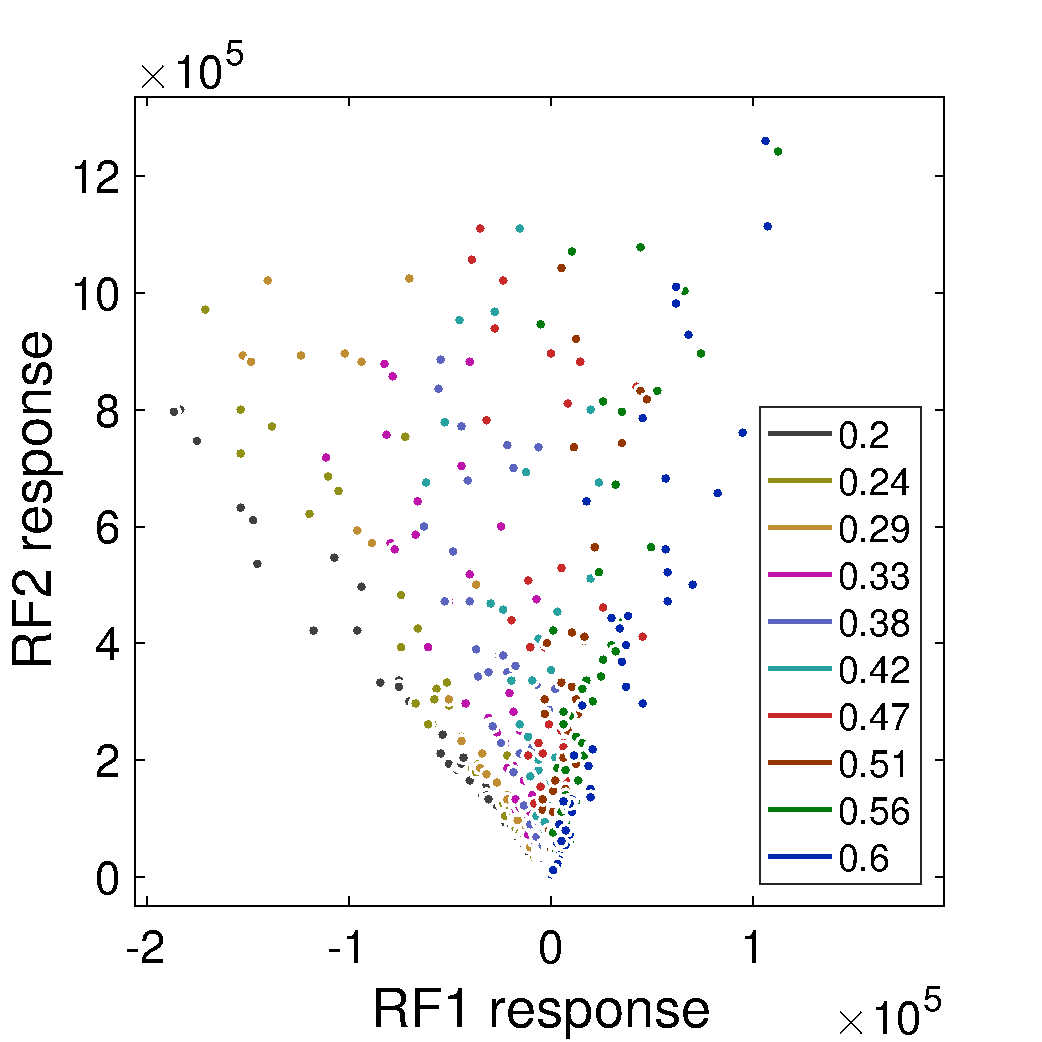
\includegraphics[width=\textwidth, trim={0 0 0 1.5cm},clip]{../FiguresDraft4/Figure11/Figure11_a.pdf}
        \label{fig:case2IsomerizationEstimates}
    \end{subfigure}
        \begin{subfigure}[b]{0.22 \textwidth}
        \caption{\centering{RF responses} \newline\centering{(Excitations)}}
        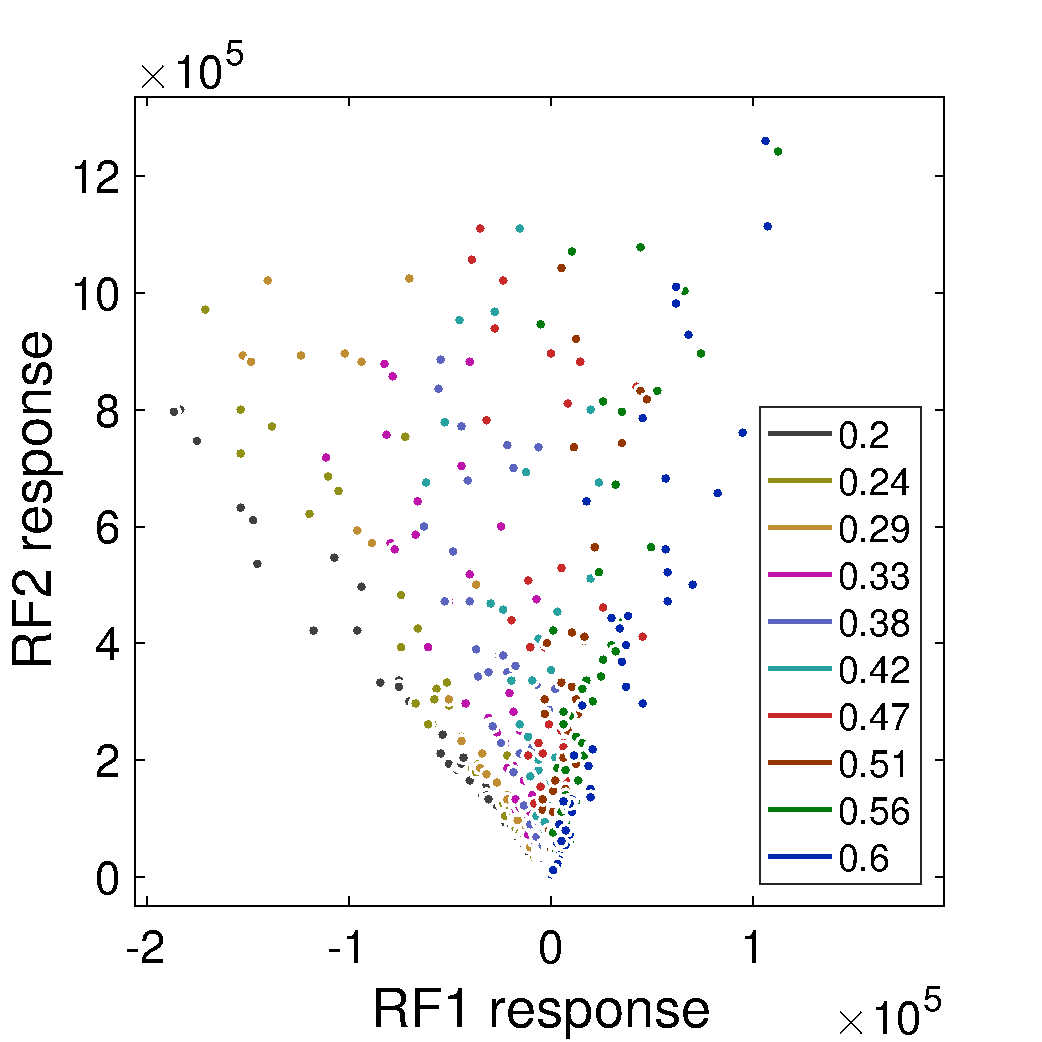
\includegraphics[width=\textwidth, trim={0 0 0 1.5cm},clip]{../FiguresDraft4/Figure11/Figure11_b.pdf}
        \label{fig:case2RFResponseIsomer}
    \end{subfigure}
            \begin{subfigure}[b]{0.22 \textwidth}
        \caption{\centering{LRV estimates}  \newline \centering{(Normalized contrast)}}
        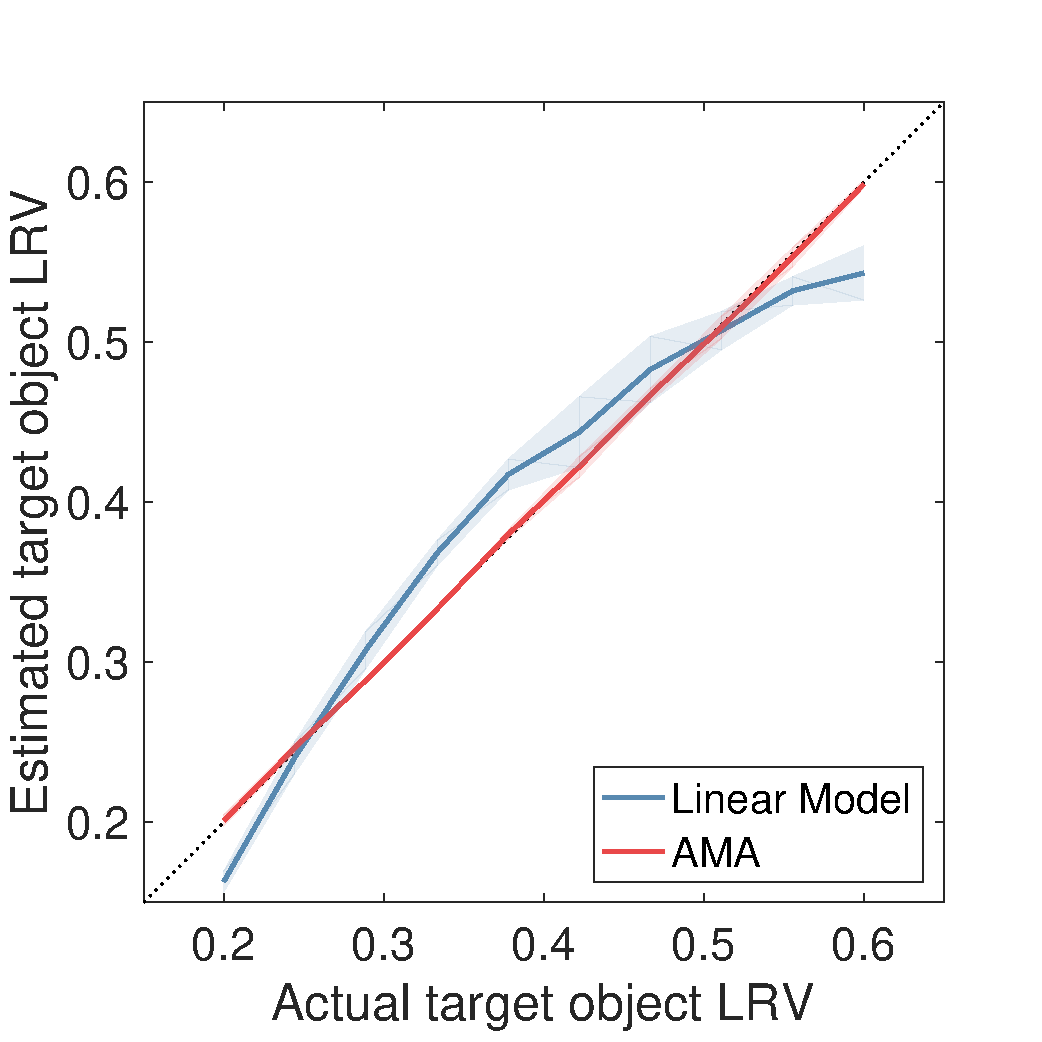
\includegraphics[width=\textwidth, trim={0 0 0 1.5cm},clip]{../FiguresDraft4/Figure11/Figure11_c.pdf}
        \label{fig:case2ContrastEstimates}
    \end{subfigure}
            \begin{subfigure}[b]{0.22 \textwidth}
        \caption{\centering{RF responses}  \newline \centering{(Normalized contrast)}}
        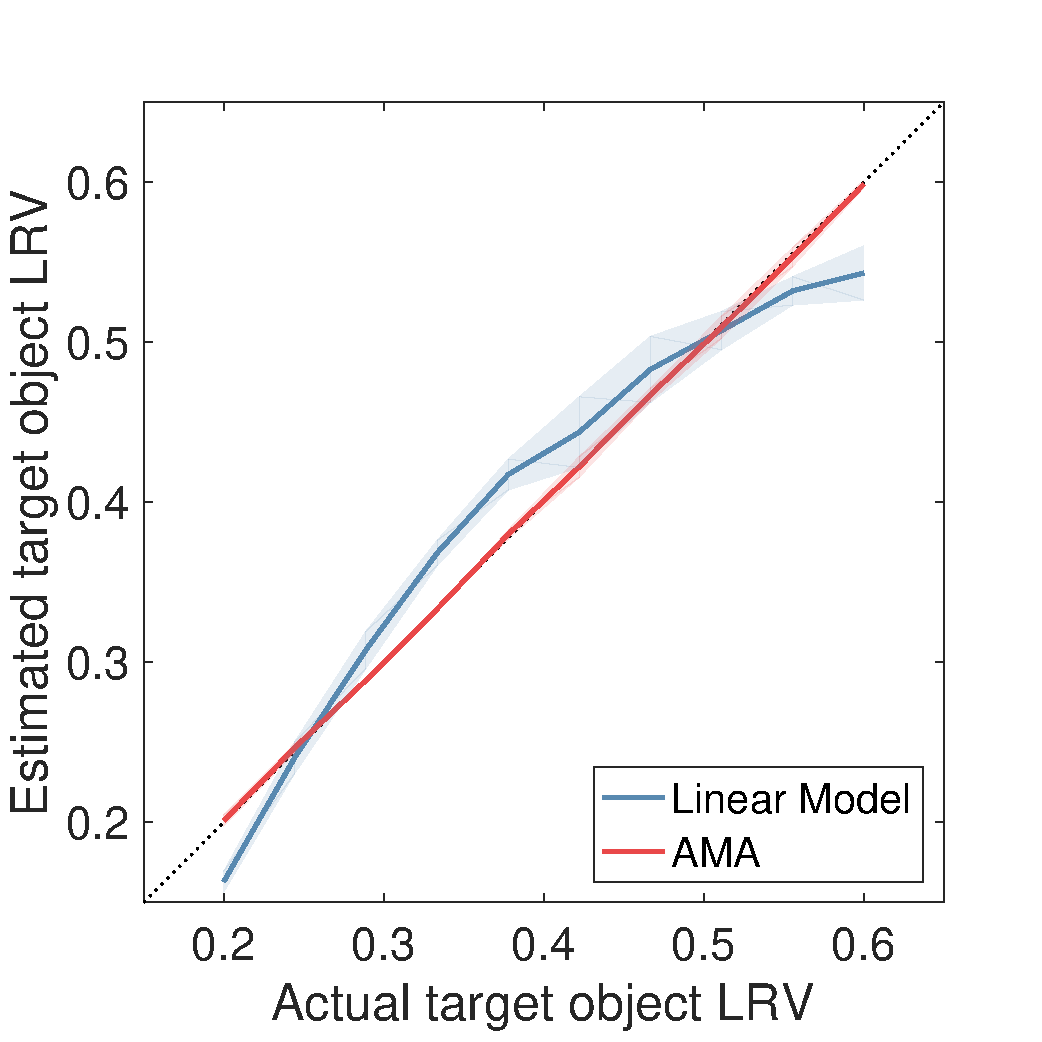
\includegraphics[width=\textwidth, trim={0 0 0 1.5cm},clip]{../FiguresDraft4/Figure11/Figure11_d.pdf}
        \label{fig:case2RFResponseContrast}
    \end{subfigure}
    \caption{{\bf Condition 2 results:} (a) Mean estimated LRV $\pm$ 1 standard deviation for images in the test set obtained using linear regression and AMA estimators, based on the cone excitations. The relative RMSE is high (41.4\% for linear regression and 31.3\% for AMA based estimation). (b) Cone isomerizations projected on AMA receptive fields calculated using cone excitations. (c) Mean estimated LRV $\pm$ 1 standard deviation for images in the test set obtained using linear regression and AMA estimators, based on the contrast normalized cone excitations. The relative RMSE of estimation is 9.3\% for linear regression and 1.1\% for AMA based estimator. (d) The contrast normalized cone excitations projected along the first two AMA receptive fields. The receptive fields were learned using AMA and the contrast normalized cone excitations. For Condition 2, the response corresponding to individual image patches at each LRV level separates much better when the input is contrast normalized cone excitations rather than the cone excitations themselves.}
\label{fig:Condition2}
\end{figure}

\subsection{Condition 2}

Condition 2 introduces variation in the spectral power distribution of the light sources.
This variation makes the task more difficult, because it causes more variation in cone excitations due to factors other than the target object LRV.
Figure~\ref{fig:Condition2}(a,b) show the results when we learned and evaluated the performance of AMA on the cone excitations.
Performance is poor.
Indeed, on average the estimates deviate considerably from the true LRV, as seen by the fact that the mean estimate
(red line) does not lie along the positive diagonal and by the fact that there is large estimation variability for each
value of the true LRV (as indicated by the width of the shaded red region).
For this case, linear regression is also very poor. Indeed, the linear regression estimates are essentially the same as would be obtained
by simply guessing the mean LRV of the training set (0.4).

Recall that there are two qualitatively distinct aspects to the variation in light source spectra.
One is a variation in relative spectral power distribution and the
other is a variation in overall intensity.
To separate the effect of these two aspects, we trained and evaluated AMA on the contrast normalized cone excitations.
Figure~\ref{fig:Condition2}(c,d) shows that performance improves greatly, and AMA performance is essentially perfect.
This observation is consistent with a large literature on computational color constancy that shows that when only illumination spectra are varied,
contrast-based representations provide an effective vehicle for achieving color constancy (REFS).
That same literature, however, shows that
contrast-based representations are less effective at supporting constancy when the spectra of background objects in the scene vary.
%% DHB: Need to add REFS in paragraph above.

%% Figure 12: Results for Condition 3
\begin{figure}
\centering
            \begin{subfigure}[b]{0.25 \textwidth}
        \caption{LRV estimates}
        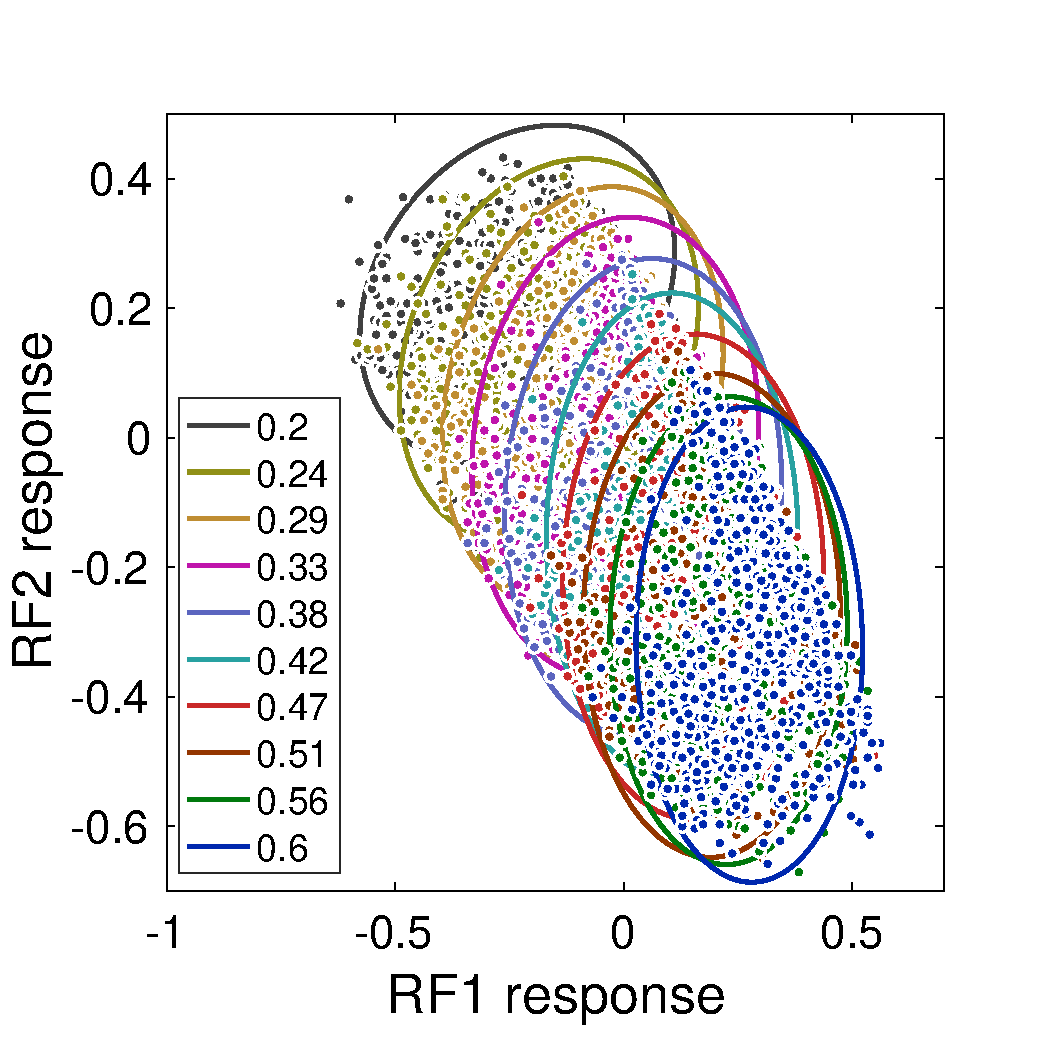
\includegraphics[width=\textwidth, trim={0 0 0 1.3cm},clip]{../FiguresDraft4/Figure12/Figure12_a.pdf}
        \label{fig:case3Estimates}
    \end{subfigure} 
        \begin{subfigure}[b]{0.26\textwidth}
        \caption{Receptive field response}
        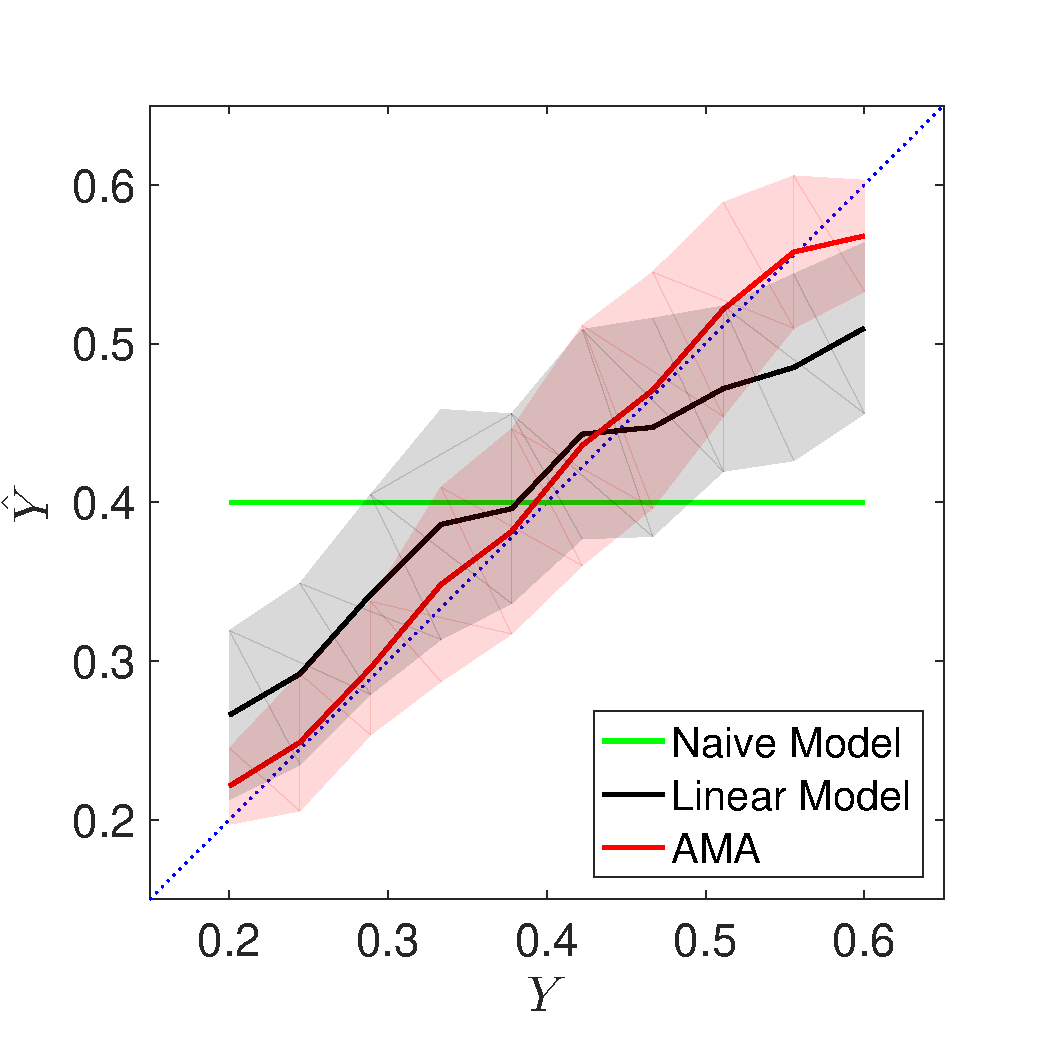
\includegraphics[width=\textwidth, trim={0 3mm 0 15mm},clip]{../FiguresDraft4/Figure12/Figure12_b.pdf}
        \label{fig:case3RFResponse}
    \end{subfigure}
    \begin{subfigure}[b]{0.4 \textwidth}
	\caption{AMA receptive fields}
	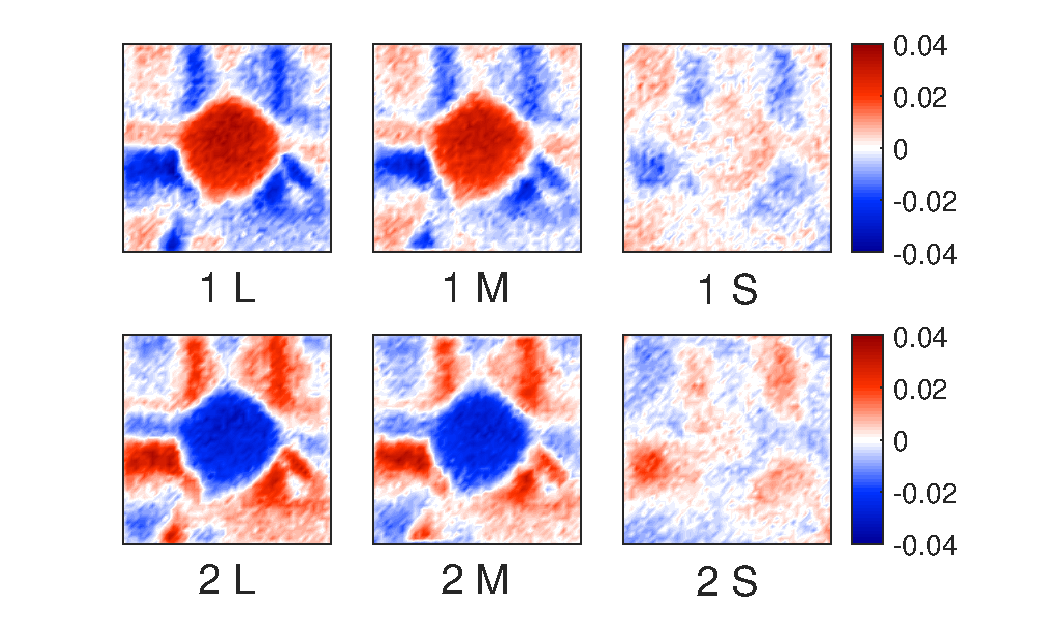
\includegraphics[width=1.0\textwidth, trim={0.2cm -0.cm 0 0.3cm}]{../FiguresDraft4/Figure12/Figure12_c.pdf}
	\label{fig:case3RFs}
    \end{subfigure}
    \caption{{\bf Condition 3 results:} (a) Mean estimated LRV $\pm$ 1 standard deviation for images in the test set obtained using linear regression and AMA estimators, based on the contrast normalized cone excitations. The relative RMSE is 22.9\%  for linear regression and 13.0\% for AMA. (b) Contrast normalized cone excitations for the training set projected along the first two AMA receptive fields. (c) First two AMA receptive fields learnt using the contrast normalized cone excitations.}
\label{fig:Condition3}
\end{figure}
%% Panel b shows training set projections, right?
%% VS: Yes

\subsection{Condition 3}

Condition 3 introduces variation in the reflectance spectra of the background objects.
This condition models the full real-world spectral variation that is most relevant for the computational problem of luminance constancy.
We again trained and evaluated AMA for labeled images patches, using the contrast normalized cone excitations.
The LRV estimates obtained via AMA are more variable and less accurate than for the previous conditions (Figure~\ref{fig:case3Estimates}).
None-the-less, the estimates provide useful information about the target LRV.
Indeed, on average the estimates track the true LRV, as seen by the fact that the mean estimate
(red line) lies along the positive diagonal.
The increased estimation variability is indicated by the increased width of the shaded red region, relative to its width for the Condition 1 and 2 results.
Performance of the baseline linear regression method (also evaluated using contrast normalized cone excitations) is worse than that of the AMA-based estimates.

Figure~\ref{fig:case3RFResponse} shows the responses of the first two AMA linear receptive fields for training stimuli.
Although the responses vary systematically with target object LRV, there is considerable overlap in the receptive field responses for stimuli having different LRV values.
This overlap is the combined effect of the variation in the illumination and background surface spectra.
Recall, however, that performance is based on six rather than two receptive fields.
Inclusion of more receptive fields reduces the ambiguity that is seen when we visualize the responses of just the first two receptive fields.
%% DHB: It might be natural here to show a plot of relative RMSE versus number of receptive fields, and for the best number of receptive
% fields of relative RMSE versus size of training set.  We want to persuade the reader that we are at asymptote.

Figure~\ref{fig:case3RFs} shows the first two receptive fields learned for Condition 3.
%% DHB: We need to write something interpretive about the RF structure shown in panel c.

%% DHB; We were going to vary the number of secondary reflections modeled in the rendering for one of the conditions, to
% separate the two possible sources of influence of the background surfaces.

\section{Discussion} \label{Discussion}

\subsection{Summary}

In this paper, we studied luminance constancy using naturalistic images.
We used a software pipeline, which was developed for this work, to render datasets of multispectral images from scene descriptions.
Because we rendered the images, we were able to label each image by the luminance reflectance value (LRV) of a target object.
Across scenes, we varied the LRV of the target object, its relative surface reflectance spectrum, 
the spectral power distributions of the light sources, and the reflectance spectra of the background objects in the scene.
These variations were based on statistical models of natural surface reflectance and illumination spectra.
We used the labeled datasets to learn estimators for the target object LRV.
We studied the performance of these estimators as we systematically manipulated the 
spectral variation in the datasets.

% Figure Error Bar Graphs
\begin{figure}
\centering
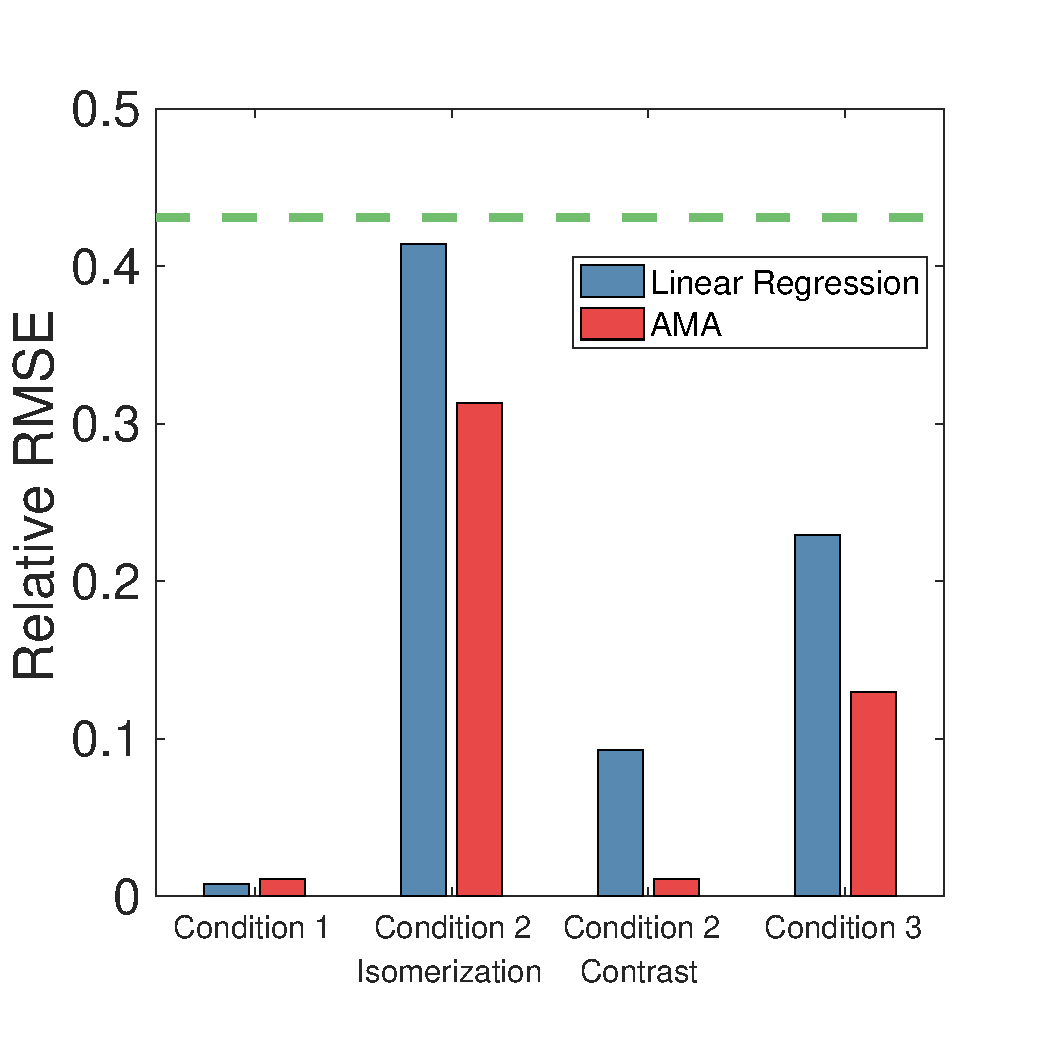
\includegraphics[width=0.3\textwidth]{../FiguresDraft4/Figure13/Figure13_a.pdf}
\caption{{\bf Summary of luminance constancy performance:} The plot shows the relative RMSE estimation error for each method and condition.The relative RMSE is the square root of the mean of the squared difference between the estimated and true LRV divided by the true LRV. The mean is taken over all stimuli in the test set.}
 \label{fig:barGraphs}
\end{figure}

Figure~\ref{fig:barGraphs} summarizes our main findings.
It plots the overall relative root mean squared estimation error (relative RMSE) for each condition. 
In Condition 1, where only the relative target object spectrum varies, luminance constancy poses an easy computational problem,
and performance is essentially perfect for both the baseline linear regression and AMA methods.
In Condition 2, where the spectral power distribution of the illumination also varies, the problem of luminance constancy is more difficult.
Indeed, neither of our methods performs well when they directly act on the cone excitations.
Performance with both methods improves greatly when the cone excitations are contrast normalized. 
Indeed, AMA performance for this case is, as in Condition 1, essentially perfect.
Linear regression does less well, in part because it only has access to cone excitations at image locations
corresponding to the target object.
Condition 2, however, does not include scene-to-scene variation in the background surface reflectances,
as occurs in natural viewing.
The results for Condition 3 show performance when we add such variation.
Performance here represents the overall level of luminance constancy that our methods achieve for the
most realistic condition that we tested.
In this case, AMA-based estimates of target object LRV are, on average, within 13\% (relative RMSE) of the true value.
Note that introduction of variation in the background surfaces makes the luminance constancy problem substantially harder,
because variation in the background surfaces reduces the reliability of the light reflected from these
surfaces as a cue to the spectral power distribution of the illuminant.

\subsection{Use of Virtual Scenes}

AMA has been used in conjunction with database of labeled natural images to analyze the estimation of defocus blur,
binocular disparity and retinal image motion (refs).
Here we used labeled images rendered from virtual scene descriptions.
The use of rendered images has advantages and disadvantages.

As we noted in the introduction, supervised learning requires large labeled datasets.
These are not readily available  for the study of how to estimate correlates of object surface reflectance.
In particular, to obtain ground truth information about the reflectance of objects in a natural image, it is necessary to
make an independent of the illumination impinging on each object.
Although this can be done by inserting a small number of discretely spaced reflectance standards into the scene, 
interpolating to locations between such standards requires strong assumptions.
The use of rendered images allows us to work with large numbers of labeled images where object reflectance
is precisely known at each pixel.

A second advantage of using rendered images is that we can control the variation in distinct
scene factors that might affect the difficulty of the estimation problem.
This allows study of the individual effect of each factor as well as their combined effect.
Here, we exploited this to systematically introduce variation in the relative target object reflectance
spectrum, the spectrum of the illumination, and the reflectance spectrum of the background objects.
This allowed us to quantify how each of these variations limits LRV estimation.
We believe the basic approach can be extended to include parametric control over the amount
of variation of different factors as well as to include variation in additional factors (see below).
%% DHB: Update if we add additional analyses as per some of the comments above.

At the same time, it is important to recognize limitations of the rendered image approach.
Virtual rendered scenes are not guaranteed to capture all of the task relevant
variation that occurs in real scenes.
Indeed, even casual inspection of our images reveals that they are rendered and not real.
Computer graphics is getting better, however, and we expect that the gap between
virtual and natural image databases will steadily close.
Indeed, carefully constructed graphics images are now quite difficult to differentiate
from real images.
%% DHB: Might be able to reference Farid's recent book on this point.

Our use of virtual images relies on datasets that characterize the statistical variation
in object reflectance and natural illumination spectra.
We believe these datasets provide reasonable approximations.
None-the-less, they can be extended and improved.
For example, the dataset of illuminations does not include the artificial illuminations
that we now live much of our lives under.
The surface reflectance datasets capture constraints on naturally occurring reflectance
functions, but the surfaces in the datasets were not sample the environment in a manner that
characterizes the relative frequency of different reflectance spectra in natural viewing.
Future work with virtual image datasets will benefit from targeted efforts to characterize
the natural statistics of the scene components that are varied.
Under the assumption that combination of different scene factors (e.g. surface reflectances
and illuminations) is independent, the virtual image approach modularizes the study
of variation in natural scenes.

\subsection{Future Directions}
In the work presented here, we incorporated spectral variation into our statistical model
of naturalistic scenes.
It is natural to begin with spectral variation, because this variation is at the heart of
what makes luminance constancy a rich computational problem.
In natural scenes, however, there are other sources of variation that add additional
richness.
These include variation in non-spectral properties of objects and lighting in the scene, including
object texture, material, and shape as well as lighting geometry.
The methods we developed here may be generalized to study the effects of variation
in these factors.
The basic approach would be to incorporate the variation into the generation of the
scenes and again learn estimators from the corresponding labeled images.
A challenge for this approach will be to thoughtfully control the increase in problem
complexity, both to keep compute time feasible and to ensure that it is possible to
extract meaningful insight from the results.

Luminance constancy is a special case of the more general problem of color constancy.
The approach we developed here could be generalized to the estimation of additional
surface reflectance descriptors, such as object hue or chroma.
As with LRV, these descriptors would be defined by the light reflected from an object's
surface   under a standard illuminant.
A further advance would be to develop methods for learning receptive fields that are
optimal for multivariate estimation problems.
With such methods one could directly estimate three-dimensional color descriptors.

\subsection{Linking to Human Performance}

An important motivation for studying the computational problem of luminance constancy
is to gain insight about human vision.
The approach we developed can be used to make predictions of how humans would
perform in a psychophysical task that probes the visual representation of object LRV.
For example, one could study discrimination thresholds for target LRV using the
stimuli that were generated with the methods used here.
More specfically, we could ask how LRV discrimination thresholds are impacted by 
spectral variation in the illuminant, the background objects, and in the target object itself.
Comparing human thresholds with the precision of AMA-based estimates would then
allow inferences about how well human observers make use of the information available
in the images for performing LRV discrimination.
We think experiments and analyses along these lines represent an important future direction.
By coupling the experiments and analyses we hope to advance, in a principled and controlled manner,
our understanding of how we see objects in the real world .

\bibliography{references}
\bibliographystyle{jovcite}

\end{document}

